\documentclass{easychair}

\usepackage{doc}
\usepackage{graphicx}
\let\Bbbk\relax
\usepackage{latexsym,amsmath,amsfonts,amssymb,epsfig}
\usepackage{ifthen}
\usepackage{seqsplit}
\usepackage{url}
\usepackage{booktabs}
\usepackage{threeparttable}
\usepackage{adjustbox}
\usepackage{comment}

% --- Algorithm packages ---
% NOTE: We use `algorithm` + `algpseudocode` (algorithmicx) because
% the Step 1..Step 6 blocks use \State / \Return / \begin{algorithmic}.
% Do NOT load algorithm2e together with algpseudocode — they conflict.
\usepackage{algorithm}
\usepackage{algpseudocode}

\usepackage{color}
\usepackage{tabularx}
\usepackage{arydshln}
\usepackage{calc}
\usepackage{amstext}
\usepackage{multicol}
\usepackage{pslatex}
\usepackage{dashbox}
\usepackage{float}
\usepackage{inconsolata}
\usepackage{multirow}
\usepackage{makecell}
\usepackage{subcaption}
\usepackage{xcolor,listings}
\usepackage{enumitem}
\usepackage{placeins}
\usepackage{pgfplots}
\pgfplotsset{compat=1.18}
\usetikzlibrary{patterns}

% --- Custom macros ---
\newcommand{\Hf}{\mathsf{H}}
\newcommand{\HkdfExtract}{\mathsf{HKDF\text{-}Extract}}
\newcommand{\HkdfExpand}{\mathsf{HKDF\text{-}Expand}}
\newcommand{\KDF}{\mathsf{KDF}}
\newcommand{\DHf}{\mathsf{DH}}
\newcommand{\AEnc}{\mathsf{Enc}}
\newcommand{\ADec}{\mathsf{Dec}}
\newcommand{\KemKeyGen}{\mathsf{KeyGen}}

% --- Variant naming macros (uniform "Section X.Y~\cite{pq-edhoc-draft}") ---
% Use \VarSec{2} or \VarSec{3.2} ... in body text whenever you refer to a
% variant of the proposed protocol. This guarantees a single, uniform style
% paper-wide and makes future edits trivial.
\newcommand{\VarSec}[1]{Section~#1~\cite{pq-edhoc-draft}}
% Short variant (no citation), useful inside captions/tables where the
% citation would already have been introduced or is redundant:
\newcommand{\VarSecShort}[1]{Section.~#1}

\usepackage[
    n, operators, advantage, sets, adversary, landau, probability,
    notions, logic, ff, mm, primitives, events, complexity,
    asymptotics, keys]{cryptocode}

\sloppy
\renewcommand{\arraystretch}{1.3}

\newcommand{\EDHOC}{\textsf{EAP-EDHOC-PQ}}
\newcommand{\Hash}{\sf{H}}
\newcommand{\Code}[1]{\ttfamily #1}
\newcommand{\HKDFextract}{\mathrm{HKDF\text{-}Extract}}
\newcommand{\HMAC}{\mathrm{HMAC\text{-}SHA256}}
\newcommand{\SHA}{\mathrm{SHA256}}
\newcommand{\X}{\mathsf{X25519}}
\newcommand{\Encaps}{\mathsf{KEM.Encaps}}
\newcommand{\Decaps}{\mathsf{KEM.Decaps}}
\newcommand{\Ed}{\mathsf{Ed25519}}
\newcommand{\CBOR}{\mathsf{CBOR}}
\newcommand{\Concat}{\mathbin{\|}}

\title{EAP-EDHOC-PQ: Design, Formal Analysis, and Empirical Evaluation of Post-Quantum EDHOC over EAP for IoT Network Access Authentication}

\author{
Adi Panca Saputra Iskandar\inst{1,2}
\and
Ilsun You\inst{2}
}

\institute{
Kookmin University, Seoul, Korea\\
\email{adipancaiskandar@gmail.com, ilsunu@gmail.com}
\and
Udayana University, Bali, Indonesia\\
}

\authorrunning{Iskandar dkk.}
\titlerunning{EAP-EDHOC-PQ: Desain, Analisis, dan Evaluasi}

\begin{document}

\maketitle

\begin{abstract}
\emph{Internet of Things} (IoT) menopang berbagai operasi e-bisnis ---
mesin penjual otomatis berjaringan, terminal \emph{point-of-sale} (POS)
cerdas dan swalayan, label rak elektronik, \emph{beacon} ritel cerdas,
\emph{charger} kendaraan listrik (EV), meteran parkir cerdas, pelacak
armada dan rantai dingin, serta \emph{gateway} sensor industri ---
yang seluruhnya bergabung ke jaringan Wi-Fi atau non-3GPP melalui
\emph{Extensible Authentication Protocol} (EAP) dan harus tetap aman
terhadap penyerang kuantum di masa depan. \emph{Ephemeral
Diffie--Hellman over COSE} (EDHOC, RFC~9528) adalah pertukaran kunci
terotentikasi yang ringan untuk perangkat terbatas, dan
\emph{Internet-Draft} \texttt{draft-papon-lake-pq-edhoc}
mendefinisikan lima varian otentikasi pasca-kuantum (PQ) di atas
ML-KEM dan ML-DSA. Namun, dampak gabungan dari pembesaran kunci PQ,
fragmentasi EAP, dan transportasi RADIUS pada \emph{deployment} AAA
nyata belum dikuantifikasi, dan analisis formal varian PQ-EDHOC
yang terintegrasi dengan EAP masih jarang. Kami menutup celah ini
dengan mengusulkan \emph{EAP-EDHOC-PQ}, metode EAP terpadu yang
menanamkan kelima varian PQ-EDHOC. Kami memverifikasi otentikasi
mutual, kerahasiaan kunci sesi, \emph{forward secrecy}, dan
ketahanan \emph{replay} di bawah penyerang Dolev--Yao dalam
ProVerif, dan secara empiris mengevaluasi desain pada \emph{testbed}
IoT heterogen (Raspberry~Pi~5 sebagai \emph{Initiator}, MacBook~Air~M3
sebagai \emph{Authenticator}/\emph{Responder}) pada tiga
\emph{deployment}: Non-EAP, EAP-Standalone, dan EAP/RADIUS penuh
dengan FreeRADIUS. Pada ukuran fragmen 256-\emph{byte} yang
konservatif, total \emph{byte} kawat berkisar dari $7{,}031$ hingga
$11{,}614$ ($29$ hingga $48$ fragmen) dan waktu \emph{handshake}
jalur AAA dari $56$~ms hingga $440$~ms antar varian. Model energi
orde-pertama yang diturunkan dari pengukuran yang sama menunjukkan
bahwa tunggu I/O akibat fragmentasi --- bukan kriptografi ---
mendominasi energi per-\emph{handshake} pada \emph{endpoint}
kelas-IoT. Hasil ini mengkuantifikasi \emph{trade-off} antara
kekuatan otentikasi, jumlah \emph{round-trip}, dan fragmentasi,
serta memberikan panduan \emph{deployment} konkret untuk otentikasi
akses jaringan PQ pada pengaturan IoT \emph{e-business}.

\flushleft{{\bf Kata Kunci:} Keamanan E-Bisnis, IoT, EDHOC, EAP,
Kriptografi Pasca-Kuantum, ML-KEM, ML-DSA, ProVerif, FreeRADIUS}
\end{abstract}


%=========================================================================
\section{Pendahuluan}
\label{Introduction}
%=========================================================================
IoT semakin tertanam dalam alur kerja e-bisnis sehari-hari.
Contoh \emph{endpoint} kritis-bisnis yang representatif meliputi
\emph{(i)}~mesin penjual otomatis berjaringan yang menerima pembayaran
nirtunai dan kode QR;
\emph{(ii)}~terminal \emph{point-of-sale} (POS) cerdas dan swalayan;
\emph{(iii)}~label rak elektronik dan \emph{beacon} ritel cerdas yang
mendorong keterlibatan pelanggan di toko;
\emph{(iv)}~\emph{charger} kendaraan listrik (EV) dan meteran parkir
cerdas yang dioperasikan ritel atau pemerintah kota;
\emph{(v)}~pelacak armada dan sensor rantai dingin yang memantau
kondisi logistik; dan
\emph{(vi)}~sensor industri terhubung dan \emph{gateway}
\emph{programmable logic-controller} (PLC) yang memasok jalur
pemeliharaan prediktif di lantai pabrik.
Secara komersial, masing-masing perangkat ini adalah \emph{endpoint}
bisnis kecil yang menangani data pembayaran, perilaku pelanggan,
atau telemetri operasional, sehingga harus didaftarkan dan
diotentikasi sebelum bertukar data dengan \emph{back-office}. Saat
\emph{endpoint} tersebut bergabung ke jaringan perusahaan ---
paling sering via Wi-Fi atau akses non-3GPP lainnya ---
\emph{otentikasi akses jaringan} adalah lini pertahanan pertama yang
menetapkan identitas perangkat, menurunkan kunci sesi, dan
menggerbangi perangkat ke lalu lintas produksi. EAP~\cite{RFC3748}
menyediakan kerangka dominan untuk tugas ini: digunakan oleh
IEEE~802.1X, Wi-Fi WPA2/3-Enterprise, dan 5G-AKA, dan biasanya
berjalan di atas \emph{backend} RADIUS/Diameter dengan \emph{server}
\emph{Authentication, Authorization and Accounting} (AAA) pusat
yang membuat keputusan otentikasi akhir.

Di antara banyak metode EAP, EAP-TLS~\cite{RFC5216},
EAP-AKA~\cite{RFC4187} dan EAP-PSK~\cite{RFC4764} adalah yang paling
luas digunakan. Namun untuk perangkat IoT bersumber daya terbatas,
EAP-TLS mahal dalam jumlah \emph{byte} di kawat dan rantai
sertifikat~\cite{FVW24,LopezGomez2026}. EDHOC~\cite{RFC9528,RFC9529}
adalah pertukaran kunci Diffie--Hellman terotentikasi yang ringan
menggunakan \emph{Concise Binary Object Representation}
(CBOR)~\cite{RFC8949} dan \emph{CBOR Object Signing and Encryption}
(COSE)~\cite{RFC9052}, dirancang untuk jaringan dengan sumber daya
terbatas dan distandarkan oleh kelompok kerja IETF LAKE~\cite{LAKE}.
Kerja terbaru mengusulkan penanaman EDHOC sebagai metode
EAP~\cite{RFC-EAP-EDHOC,LopezGomez2026}, yang membawa \emph{flight}
kompak EDHOC ke akses jaringan berbasis AAA arus utama.

Pada saat yang sama, algoritma Shor~\cite{shor1994algorithms}
mengancam setiap \emph{deployment} kurva eliptik yang digunakan saat
ini. Walaupun komputer kuantum yang relevan secara kriptanalitik
belum tersedia, model penyerang \emph{harvest-now, decrypt-later}
sudah menjadi kekhawatiran terdokumentasi bagi data bisnis berumur
panjang seperti catatan pembayaran dan telemetri rantai pasok, dan
memotivasi memulai transisi sebelum mesin tersebut hadir. NIST telah
menstandarkan ML-KEM (FIPS~203)~\cite{FIPS203} dan ML-DSA
(FIPS~204)~\cite{FIPS204} sebagai pengganti pasca-kuantum lini
pertama. Regulator di Prancis~\cite{ANSSI} dan
Jerman~\cite{TR-02102-1} serta kelompok kerja IETF
PQUIP~\cite{PQUIP} merekomendasikan kombinasi \emph{hybrid}
PQ/tradisional selama periode transisi. Varian pasca-kuantum dari
EDHOC (\texttt{draft-papon-lake-pq-edhoc}) sedang dalam spesifikasi
aktif~\cite{pq-edhoc-draft} dan mendefinisikan lima mode otentikasi
pada Section~2, 3.2, 3.3, 3.4, dan 3.5; analisis lanjutan telah
mengevaluasi EDHOC tahan-kuantum pada
mikrokontroler~\cite{FTK+25,FKF25}.

Yang belum dipahami adalah apa yang terjadi ketika varian PQ-EDHOC
ini diangkut oleh \emph{EAP dalam pengaturan AAA nyata}. EAP
mendefinisikan MTU minimum hanya $1020$ oktet dan mewajibkan alur
\emph{lock-step} dengan ACK fragmen untuk \emph{payload} yang lebih
besar dari itu~\cite{RFC3748,RFC9191}. \emph{Cipherteks} ML-KEM dan
tanda tangan ML-DSA mendorong pesan EDHOC individu ke kisaran
multi-kilobyte, sehingga setiap pesan \emph{handshake} menimbulkan
beberapa fragmen dan \emph{round-trip} tambahan ujung-ke-ujung
antara \emph{peer} EAP, \emph{authenticator}, dan \emph{server} AAA.
Studi empiris EDHOC sebelumnya~\cite{FVW24,FTK+25,FKF25} mengevaluasi
EDHOC \emph{peer-to-peer} dan tidak menjalankan jalur EAP/RADIUS;
kerja EAP-EDHOC sebelumnya~\cite{RFC-EAP-EDHOC,LopezGomez2026}
berfokus pada himpunan primitif klasik.

\subsection{Penelitian Terkait}
\label{sec:related-work}
Kerja kami berada di persimpangan empat alur: (i) kerangka EAP itu
sendiri dan metode-metode
kanoniknya~\cite{RFC3748,RFC5216,RFC4187,RFC4764}; (ii) EDHOC dan
integrasinya dengan EAP~\cite{RFC9528,RFC9529,LAKE,RFC-EAP-EDHOC,LopezGomez2026,FVW24};
(iii) pertukaran kunci pasca-kuantum dan \emph{hybrid}, termasuk
FIPS~203/204~\cite{FIPS203,FIPS204}, ETSI TS~103~744~\cite{TS103744},
PQXDH~\cite{PQXDH,FG24}, PQ Noise~\cite{ADH+22}, IKEv2
\emph{hybrid}~\cite{RFC9370}, dan TLS~1.3 \emph{hybrid}~\cite{TLS};
serta (iv) analisis formal dan komputasional EDHOC seperti pada
~\cite{KDL+21,NSB21,CP22,GM23,JKK+23,Fer24,PSM+24}.
\emph{Internet-Draft} otentikasi EDHOC berbasis-KEM~\cite{pocero} dan
\emph{draft} PQ-EDHOC tanda-tangan/KEM~\cite{pq-edhoc-draft} adalah
pendahulu terdekat dari proposal kami, dan notasi KEM yang lebih
kuat seperti pada~\cite{CDM24} memotivasi mengapa \emph{handshake}
yang diotentikasi-KEM layak mendapat perlakuan simbolis yang cermat.

\subsection{Celah Penelitian}
\label{sec:gap-research}
Meskipun ada kemajuan substansial pada masing-masing alur tersebut,
empat celah masih ada. \emph{Pertama}, dampak pembesaran
kunci/cipherteks PQ pada fragmentasi EAP di bawah MTU minimum EAP
$1020$ oktet belum dikuantifikasi. \emph{Kedua}, analisis simbolis
formal varian PQ dari EAP-EDHOC belum dipublikasikan, dan model
ProVerif yang ada menargetkan EDHOC klasik~\cite{NSB21,JKK+23}.
\emph{Ketiga}, evaluasi empiris PQ-EDHOC sejauh ini menargetkan
EDHOC \emph{peer-to-peer} atau mikrokontroler tanpa \emph{backend}
AAA nyata~\cite{FTK+25,FKF25}. \emph{Keempat}, mode-mode otentikasi
PQ-EDHOC yang berbeda (hanya-KEM, hanya-tanda-tangan, dan
\emph{hybrid}) belum dibandingkan secara seragam pada
\emph{deployment} dengan EAP dan \emph{server} AAA nyata seperti
FreeRADIUS.

\subsection{Kontribusi}
\label{sec:contribution}
Kami menjawab celah-celah tersebut dengan kontribusi berikut. Di
seluruh makalah, kami merujuk lima varian otentikasi dari
\texttt{draft-papon-lake-pq-edhoc} dengan nomor \emph{section}
\emph{draft}-nya, yaitu \VarSec{2}, \VarSec{3.2}, \VarSec{3.3},
\VarSec{3.4} dan \VarSec{3.5}; tata nama ini digunakan secara seragam
pada setiap algoritma, tabel, dan gambar.
\begin{itemize}[leftmargin=1.2em,itemsep=2pt,topsep=2pt]
\item Kami menspesifikasikan \textbf{EAP-EDHOC-PQ}, sebuah metode EAP
terpadu yang menanamkan kelima varian otentikasi PQ-EDHOC
dari~\cite{pq-edhoc-draft} --- mode tiga-\emph{flight} terotentikasi
KEM secara implisit (\VarSec{2},
Section~\ref{sec:variant-s2}); mode tiga-\emph{flight} tanda-tangan+KEM
(\VarSec{3.2}, Section~\ref{sec:variant-s32}); dan tiga varian
\emph{hybrid} empat-\emph{flight} (\VarSec{3.3}, \VarSec{3.4} dan
\VarSec{3.5}, Section~\ref{sec:variant-s33}--\ref{sec:variant-s35}) ---
di atas EAP dan RADIUS.
\item Kami menyediakan \textbf{model ProVerif} untuk kelima varian dan
membuktikan otentikasi mutual, kerahasiaan kunci sesi,
\emph{forward secrecy}, dan ketahanan terhadap \emph{replay} di bawah
penyerang Dolev--Yao (Section~\ref{security-analysis}).
\item Kami memberikan \textbf{evaluasi empiris} pada \emph{testbed}
nyata dengan \emph{deployment} Non-EAP, EAP-Standalone, dan EAP/RADIUS
penuh (FreeRADIUS) pada ukuran fragmen konservatif 256 \emph{byte},
mengukur fragmentasi, waktu pemrosesan, \emph{overhead}, dan latensi
per-operasi (Section~\ref{performance-evaluation}).
\item Kami menurunkan \textbf{panduan \emph{deployment}} yang konkret:
varian mana yang meminimalkan \emph{byte} kawat, mana yang meminimalkan
\emph{round-trip}, dan bagaimana jalur AAA memperbesar biaya mode
\emph{hybrid} empat-\emph{flight} (Section~\ref{discussion}).
\end{itemize}

Sisanya makalah disusun sebagai berikut.
Section~\ref{pleminary} memperkenalkan primitif, model EAP/RADIUS,
dan notasi. Section~\ref{proposed-design} menspesifikasikan desain
EAP-EDHOC-PQ terpadu beserta lima variannya.
Section~\ref{sec:comparison} membandingkan desain terpadu kami dengan
penyajian dua-mode asli dari~\cite{pq-edhoc-draft}.
Section~\ref{security-analysis} menyajikan analisis ProVerif.
Section~\ref{performance-evaluation} melaporkan evaluasi empiris.
Section~\ref{discussion} membahas implikasi dan keterbatasan.
Section~\ref{conclusion} menyimpulkan.


%=========================================================================
\section{Pendahuluan Teknis}
\label{pleminary}
%=========================================================================
Bagian ini menetapkan notasi, mengingat kembali primitif kriptografi
yang digunakan, merangkum EDHOC dan EAP, serta memperkenalkan model
ancaman. Tabel~\ref{tab:abbr} mendaftar singkatan yang dipakai di
seluruh makalah.

\begin{table}[h]
\centering
\scriptsize
\caption{Singkatan dan notasi yang dipakai di seluruh makalah
(termasuk semua simbol pada Algorithm~\ref{alg:step1}--\ref{alg:step6}
di Section~\ref{proposed-design}).}
\label{tab:abbr}
\setlength{\tabcolsep}{4pt}
\begin{tabularx}{\linewidth}{@{}l X l X@{}}
\toprule
\textbf{Simbol} & \textbf{Arti} & \textbf{Simbol} & \textbf{Arti} \\
\midrule
\multicolumn{4}{l}{\textit{Protokol dan kerangka}} \\
EAP    & Extensible Authentication Protocol (RFC~3748) & EDHOC  & Ephemeral Diffie--Hellman over COSE (RFC~9528) \\
AAA    & Authentication, Authorization, Accounting (RADIUS/Diameter) & NAS    & Network Access Server (merelai EAP antara \emph{peer} dan AAA) \\
RADIUS & Remote Authentication Dial-In User Service (RFC~2865) & CBOR   & Concise Binary Object Representation (RFC~8949) \\
COSE   & CBOR Object Signing and Encryption (RFC~9052) & MTU    & Maximum Transmission Unit \\
LAKE   & kelompok kerja IETF untuk \emph{Lightweight AKE} & & \\
\midrule
\multicolumn{4}{l}{\textit{Primitif kriptografi}} \\
KEM    & Key Encapsulation Mechanism & ML-KEM & Module-Lattice KEM (FIPS~203) \\
ML-DSA & Module-Lattice Digital Signature Algorithm (FIPS~204) & DS     & skema Tanda Tangan Digital (diinstansiasi oleh ML-DSA) \\
AEAD   & Authenticated Encryption with Associated Data & HKDF   & KDF berbasis-HMAC (RFC~5869) \\
KDF    & Key Derivation Function & HMAC   & Hashed Message Authentication Code \\
MAC    & Message Authentication Code & SHA-256 & Secure Hash Algorithm, keluaran 256-bit \\
$H(\cdot)$ & fungsi \emph{hash} kriptografi (SHA-256 pada instansiasi kami) & $\KemKeyGen,\Encaps,\Decaps$ & pembangkitan kunci, \emph{encapsulation}, \emph{decapsulation} KEM \\
$\mathbf{DS.Sign},\mathbf{DS.Verify}$ & penandatanganan / verifikasi tanda tangan & $\mathbf{AEAD.Enc},\mathbf{AEAD.Dec}$ & enkripsi / dekripsi AEAD \\
\midrule
\multicolumn{4}{l}{\textit{Pihak, pengenal, dan kredensial}} \\
$I$, $R$ & EDHOC \emph{Initiator}, \emph{Responder} & $C_I$, $C_R$ & pengenal koneksi EDHOC yang dipilih $I$, $R$ \\
$ID\_CRED_I$, $ID\_CRED_R$ & pengenal kredensial $I$, $R$ & METHOD, $\mathrm{SUITES}_I$ & \emph{byte} metode EDHOC dan daftar \emph{cipher-suite} yang ditawarkan \\
$\mathrm{EAD}_i$ & \emph{External Authorization Data} pada pesan~$i$ & MSK, EMSK & \emph{Master Session Key}, \emph{Extended} MSK yang diekspor ke EAP \\
\midrule
\multicolumn{4}{l}{\textit{Material kunci per-\emph{handshake}}} \\
$sk_X, pk_X$ & kunci rahasia/publik jangka panjang pihak $X$ & $\mathrm{kem.sk}_X, \mathrm{kem.pk}_X$ & pasangan kunci KEM jangka panjang pihak $X$ \\
$\mathrm{sign.sk}_X, \mathrm{sign.pk}_X$ & pasangan kunci tanda tangan jangka panjang pihak $X$ & $\mathrm{kem.sk}_{\mathrm{eph}}, \mathrm{kem.pk}_{\mathrm{eph}}$ & pasangan kunci KEM \emph{ephemeral} yang dibangkitkan $I$ \\
$\mathrm{kem.ct}_{\mathrm{eph}}$ & \emph{cipherteks} KEM ke $\mathrm{kem.pk}_{\mathrm{eph}}$ & $\mathrm{kem.ct}_R, \mathrm{kem.ct}_I$ & \emph{cipherteks} KEM ke kunci jangka panjang $R$, $I$ \\
$\mathrm{ss}_{\mathrm{eph}}, \mathrm{ss}_R, \mathrm{ss}_I$ & \emph{shared secret} dari ketiga operasi KEM & $TH_i$ & \emph{transcript hash} EDHOC setelah pesan~$i$ \\
$PRK_{2e}$ & PRK dari $\mathrm{ss}_{\mathrm{eph}}$ & $PRK_{3e2m}$ & PRK setelah mencampur $\mathrm{ss}_R$ \\
$PRK_{4e3m}$ & PRK setelah mencampur $\mathrm{ss}_I$ (mode empat-\emph{flight}) & $PRK_{\mathrm{out}}$ & PRK \emph{exporter} yang memasok derivasi MSK/EMSK \\
$SALT_{3e2m}, SALT_{4e3m}$ & \emph{salt} pada HKDF-Extract terkait & $KEYSTREAM_2$ & \emph{keystream} XOR yang melindungi $PLAINTEXT_2$ \\
$K_3,IV_3,K_4,IV_4$ & pasangan kunci/IV AEAD untuk pesan 3 dan 4 & $MAC_i$ & tag otentikasi yang dibawa di (atau menutup) \emph{flight}~$i$ \\
$SIGNATURE_i$ & tanda tangan ML-DSA terlampir pada \emph{flight}~$i$ & $PLAINTEXT_i, CIPHERTEXT_i$ & \emph{plaintext} / \emph{cipherteks} pesan~$i$ \\
$\parallel$ & konkatenasi \emph{byte string} & & \\
\bottomrule
\end{tabularx}
\end{table}

\subsection{Primitif Kriptografi}
Kami menggunakan primitif pasca-kuantum yang distandarkan NIST.
\textbf{ML-KEM}~\cite{FIPS203} adalah mekanisme enkapsulasi kunci
aman IND-CCA2 dengan tiga algoritma
$(\KemKeyGen,\Encaps,\Decaps)$. \textbf{ML-DSA}~\cite{FIPS204} adalah
algoritma tanda tangan digital berbasis \emph{module-lattice}.
Primitif simetris mengikuti RFC~9528: SHA-256 untuk \emph{hashing},
HKDF~\cite{RFC5869} untuk derivasi kunci, dan AES-CCM (sebuah AEAD)
untuk enkripsi terotentikasi.

\subsection{EDHOC (RFC 9528)}
EDHOC adalah pertukaran kunci terotentikasi tiga-pesan (opsional
empat-pesan) yang dikodekan dalam CBOR~\cite{RFC8949,RFC9052}. Metode
kanonik Tanda-tangan--Tanda-tangan (SIG-SIG) mentransmisikan
kontribusi Diffie--Hellman \emph{ephemeral} dan mengotentikasi kedua
pihak dengan tanda tangan digital; mode Static-DH menggunakan kunci
DH jangka panjang dan menurunkan tag MAC sebagai gantinya. Analisis
keamanan terperinci pada \emph{setting} klasik diberikan
pada~\cite{NSB21,CP22,GM23,JKK+23,Fer24,PSM+24}.

\subsection{Model EAP dan RADIUS}
EAP~\cite{RFC3748} adalah protokol \emph{request/response} model
\emph{lock-step} yang berjalan di atas lapisan bawah (mis., IEEE~802.1X,
PPP, atau IKEv2). Untuk EAP-over-RADIUS, sebuah \emph{authenticator}
(biasanya \emph{gateway} atau \emph{access point}) merelai paket EAP
antara \emph{peer} dan \emph{server} AAA di dalam atribut RADIUS. Dua
properti menjadi pusat evaluasi kami. \emph{(a)} Implementasi EAP
dapat mengasumsikan MTU hanya $1020$ oktet dari lapisan bawah, dan
EAP sendiri tidak menyediakan fragmentasi; metode EAP yang pesannya
melampaui MTU harus mengimplementasikan fragmentasi dengan ACK
eksplisit, dengan biaya \emph{round-trip}
tambahan~\cite{RFC3748,RFC9191}. \emph{(b)} Paket RADIUS dibatasi
$4096$ oktet dan membawa \emph{payload} EAP dalam beberapa AVP
\texttt{EAP-Message} berukuran $253$ \emph{byte}; pesan EAP yang
panjang karenanya melintasi batas fragmentasi EAP sekaligus batas
atribut RADIUS.

\subsection{Model Ancaman}
Kami mempertimbangkan penyerang Dolev--Yao~\cite{dolev1983security}
yang mengontrol jaringan antara \emph{peer}, \emph{authenticator},
dan \emph{server} AAA. Penyerang dapat menyisipkan, membuang,
mengurutkan ulang, mereplay, atau memodifikasi pesan apa pun dan
dapat mengompromikan kunci jangka panjang \emph{peer} selain sesi
target untuk argumen \emph{forward secrecy}. Primitif kriptografi
diidealkan sebagai fungsi simbolis sempurna, konsisten dengan model
\emph{applied-pi-calculus} ProVerif dan praktik
standar~\cite{blanchet2001proverif,blanchet2016automated,cremers2017symbolic}.


%=========================================================================
\section{Desain yang Diusulkan: EAP-EDHOC-PQ}
\label{proposed-design}
%=========================================================================
Metode \textbf{EAP-EDHOC-PQ} yang diusulkan membawa \emph{flight}
PQ-EDHOC antara \emph{peer} EAP (\emph{Initiator} EDHOC $I$, biasanya
perangkat IoT), \emph{authenticator}, dan \emph{server} AAA
(\emph{Responder} EDHOC $R$). Desain terpadu ini mendukung lima varian
otentikasi --- \VarSec{2}, \VarSec{3.2}, \VarSec{3.3}, \VarSec{3.4},
dan \VarSec{3.5} --- yang menukar mekanisme otentikasi (KEM, tanda
tangan, atau \emph{hybrid}), jumlah \emph{flight} (tiga atau empat),
dan waktu otentikasi \emph{Responder}. Gambar~\ref{fig:protocol}
merangkum alur protokol secara lengkap.
Section~\ref{sec:variant-s2}--\ref{sec:variant-s35} menjelaskan
varian-varian secara individual.

\begin{figure}[H]
    \centering
    \includegraphics[width=\linewidth]{img/simple-protocol.png}
\caption{EAP-EDHOC-PQ terpadu di atas EAP/RADIUS, lima varian:
\VarSec{2} (otentikasi \emph{Responder} implisit hanya berbasis KEM),
\VarSec{3.2} (SIG+KEM, tiga \emph{flight}),
\VarSec{3.3} (SIG+KEM, empat \emph{flight}, KEM ke $I$),
\VarSec{3.4} (KEM+KEM, otentikasi \emph{Responder} ditangguhkan), dan
\VarSec{3.5} (KEM+KEM+SIG).}
\label{fig:protocol}
\end{figure}
\FloatBarrier

% =============================================================================
% EAP-EDHOC-PQ — 6 Unified Algorithms with In-line Section Differentiators
% =============================================================================
% Each algorithm covers ALL variants from draft-papon-lake-pq-edhoc-00.
% Per-section behavior is distinguished INSIDE the algorithm using labelled
% blocks [Section 2] / [Section 3.2] / [Section 3.3] / [Section 3.4] /
% [Section 3.5], mirroring the multi-section boxes of the original diagram.
% =============================================================================

% ============================================
% STEP 1: INITIATOR — Prepare Message 1
% ============================================
\begin{algorithm}[H]
\caption{Step 1 (\emph{Initiator}) --- Menyiapkan $M_1$}
\label{alg:step1}
\textbf{Input:} Pasangan kunci PQ jangka panjang $(pk_I, sk_I)$; $\mathrm{kem.pk}_R$ milik \emph{Responder} (hanya Section~2) \\
\textbf{Output:} $M_1$
\begin{algorithmic}[1]
\Statex \textit{[All Sections]}
\State $(\mathrm{kem.sk}_{\mathrm{eph}}, \mathrm{kem.pk}_{\mathrm{eph}}) \gets \mathbf{KEM.KeyGen}()$
\Statex \textit{[Section 2 only]}
\State $(\mathrm{ss}_R, \mathrm{kem.ct}_R) \gets \mathbf{KEM.Encaps}(\mathrm{kem.pk}_R)$
\State $M_1 \gets (\mathrm{METHOD}, \mathrm{SUITES}_I, \mathrm{kem.pk}_{\mathrm{eph}}, \mathrm{kem.ct}_R, C_I, \mathrm{EAD}_1)$
\Statex \textit{[Section 3.2, 3.3, 3.4, 3.5]}
\State $M_1 \gets (\mathrm{METHOD}, \mathrm{SUITES}_I, \mathrm{kem.pk}_{\mathrm{eph}}, C_I, \mathrm{EAD}_1)$
\State \Return $M_1$
\end{algorithmic}
\end{algorithm}


% ============================================
% STEP 2: RESPONDER — Process M1, Prepare M2
% ============================================
\begin{algorithm}[H]
\caption{Step 2 (\emph{Responder}) --- Memproses $M_1$ dan menyiapkan $M_2$}
\label{alg:step2}
\textbf{Input:} $M_1$; kunci jangka panjang \emph{Responder} (KEM dan/atau penandatanganan, sesuai \emph{section}) \\
\textbf{Output:} $M_2$
\begin{algorithmic}[1]
\Statex \textit{[All Sections]}
\State $(\mathrm{ss}_{\mathrm{eph}}, \mathrm{kem.ct}_{\mathrm{eph}}) \gets \mathbf{KEM.Encaps}(\mathrm{kem.pk}_{\mathrm{eph}})$
\State $TH_2 \gets H(\mathrm{kem.ct}_{\mathrm{eph}}, H(M_1))$
\State $PRK_{2e} \gets \mathbf{EDHOC\text{-}Extract}(TH_2, \mathrm{ss}_{\mathrm{eph}})$
\State $KEYSTREAM_2 \gets \mathbf{EDHOC\text{-}KDF}(PRK_{2e}, 0, TH_2)$
\Statex \textit{[Section 2]} \Comment{implicit R-auth via $\mathrm{ss}_R$ from $M_1$}
\State $\mathrm{ss}_R \gets \mathbf{KEM.Decaps}(\mathrm{kem.sk}_R, \mathrm{kem.ct}_R)$
\State $SALT_{3e2m} \gets \mathbf{EDHOC\text{-}KDF}(PRK_{2e}, 1, TH_2)$
\State $PRK_{3e2m} \gets \mathbf{EDHOC\text{-}Extract}(SALT_{3e2m}, \mathrm{ss}_R)$
\State $MAC_2 \gets \mathbf{KDF}(PRK_{3e2m}, 2, (C_R, ID\_CRED_R, TH_2, \mathrm{EAD}_2))$
\State $PLAINTEXT_2 \gets (C_R, ID\_CRED_R, MAC_2, \mathrm{EAD}_2)$
\Statex \textit{[Section 3.2, 3.5]} \Comment{explicit R-auth via signature over $PLAINTEXT_2$}
\State $PLAINTEXT_2 \gets (C_R, ID\_CRED_R, TH_2, \mathrm{EAD}_2)$
\State $SIGNATURE_2 \gets \mathbf{DS.Sign}(\mathrm{sign.sk}_R, PLAINTEXT_2)$
\State $PLAINTEXT_2 \gets (PLAINTEXT_2 \parallel SIGNATURE_2)$
\Statex \textit{[Section 3.3]} \Comment{$MAC_2$ + signature over $MAC_2$, $MAC_2$ derived from $PRK_{2e}$}
\State $MAC_2 \gets \mathbf{KDF}(PRK_{2e}, 2, (C_R, ID\_CRED_R, TH_2, \mathrm{EAD}_2))$
\State $SIGNATURE_2 \gets \mathbf{DS.Sign}(\mathrm{sign.sk}_R, (C_R, ID\_CRED_R, TH_2, \mathrm{EAD}_2, MAC_2))$
\State $PLAINTEXT_2 \gets (C_R, ID\_CRED_R, SIGNATURE_2, \mathrm{EAD}_2)$
\Statex \textit{[Section 3.4]} \Comment{$MAC_2$ \emph{deferred} to $M_4$; $M_2$ carries no auth material}
\State $PLAINTEXT_2 \gets (C_R, ID\_CRED_R, TH_2, \mathrm{EAD}_2)$
\Statex \textit{[All Sections]}
\State $CIPHERTEXT_2 \gets PLAINTEXT_2 \oplus KEYSTREAM_2$
\State $M_2 \gets (\mathrm{kem.ct}_{\mathrm{eph}}, CIPHERTEXT_2)$
\State \Return $M_2$
\end{algorithmic}
\end{algorithm}


% ============================================
% STEP 3: INITIATOR — Process M2, Prepare M3
% ============================================
\begin{algorithm}[H]
\caption{Step 3 (\emph{Initiator}) --- Memproses $M_2$ dan menyiapkan $M_3$}
\label{alg:step3}
\textbf{Input:} $M_2$ \\
\textbf{Output:} $M_3$
\begin{algorithmic}[1]
\Statex \textit{[All Sections]}
\State $\mathrm{ss}_{\mathrm{eph}} \gets \mathbf{KEM.Decaps}(\mathrm{kem.sk}_{\mathrm{eph}}, \mathrm{kem.ct}_{\mathrm{eph}})$
\State Compute $TH_2, PRK_{2e}, KEYSTREAM_2$ and recover $PLAINTEXT_2$
\State $TH_3 \gets H(TH_2, PLAINTEXT_2, ID\_CRED_R)$
\Statex \textit{[Section 2]} \Comment{verify $MAC_2 \Rightarrow$ implicit R-auth}
\State $PRK_{3e2m} \gets \mathbf{EDHOC\text{-}Extract}(SALT_{3e2m}, \mathrm{ss}_R)$
\State Verify $MAC_2 \stackrel{?}{=} \mathbf{KDF}(PRK_{3e2m}, 2, \cdot)$
\State $(K_3, IV_3) \gets \mathbf{EDHOC\text{-}KDF}(PRK_{3e2m}, 3\text{/}4, TH_3)$
\State $MAC_3 \gets \mathbf{KDF}(PRK_{3e2m}, 6, (ID\_CRED_I, TH_3, \mathrm{EAD}_3))$
\State $SIGNATURE_3 \gets \mathbf{DS.Sign}(\mathrm{sign.sk}_I, (ID\_CRED_I, TH_3, \mathrm{EAD}_3, MAC_3))$
\State $PLAINTEXT_3 \gets (ID\_CRED_I, SIGNATURE_3, \mathrm{EAD}_3)$
\State $M_3 \gets \mathbf{AEAD.Enc}(K_3, IV_3, PLAINTEXT_3)$
\Comment{no $\mathrm{kem.ct}_R$ --- sent in $M_1$}
\Statex \textit{[Section 3.2, 3.5]} \Comment{explicit $R$-auth via signature verification; new $\mathrm{kem.ct}_R$}
\State Retrieve $\mathrm{kem.pk}_R, \mathrm{sign.pk}_R$; verify $\mathbf{DS.Verify}(\mathrm{sign.pk}_R, PLAINTEXT_2, SIGNATURE_2)$
\State $(\mathrm{ss}_R, \mathrm{kem.ct}_R) \gets \mathbf{KEM.Encaps}(\mathrm{kem.pk}_R)$
\State $PRK_{3e2m} \gets \mathbf{EDHOC\text{-}Extract}(SALT_{3e2m}, \mathrm{ss}_R)$
\State $(K_3, IV_3) \gets \mathbf{EDHOC\text{-}KDF}(PRK_{3e2m}, 3\text{/}4, TH_3)$
\State $MAC_3 \gets \mathbf{KDF}(PRK_{3e2m}, 6, (ID\_CRED_I, TH_3, \mathrm{EAD}_3))$
\State $SIGNATURE_3 \gets \mathbf{DS.Sign}(\mathrm{sign.sk}_I, (ID\_CRED_I, TH_3, \mathrm{EAD}_3, MAC_3))$
\State $CIPHERTEXT_3 \gets \mathbf{AEAD.Enc}(K_3, IV_3, (ID\_CRED_I, SIGNATURE_3, \mathrm{EAD}_3))$
\State $M_3 \gets (\mathrm{kem.ct}_R, CIPHERTEXT_3)$
\Statex \textit{[Section 3.3]} \Comment{sign $PLAINTEXT_3$ directly; no $MAC_3$; no $\mathrm{kem.ct}_R$}
\State $MAC_2 \gets \mathbf{KDF}(PRK_{2e}, 2, \cdot)$; verify $\mathbf{DS.Verify}(\mathrm{sign.pk}_R, \cdot, SIGNATURE_2)$
\State $(K_3, IV_3) \gets \mathbf{EDHOC\text{-}KDF}(PRK_{2e}, 3\text{/}4, TH_3)$
\State $PLAINTEXT_3 \gets (ID\_CRED_I, TH_3, \mathrm{EAD}_3)$
\State $SIGNATURE_3 \gets \mathbf{DS.Sign}(\mathrm{sign.sk}_I, PLAINTEXT_3)$
\State $M_3 \gets \mathbf{AEAD.Enc}(K_3, IV_3, (PLAINTEXT_3 \parallel SIGNATURE_3))$
\Statex \textit{[Section 3.4]} \Comment{no $SIG_2$ verify yet --- $R$-auth deferred to $M_4$; new $\mathrm{kem.ct}_R$}
\State $(\mathrm{ss}_R, \mathrm{kem.ct}_R) \gets \mathbf{KEM.Encaps}(\mathrm{kem.pk}_R)$
\State $PRK_{3e2m} \gets \mathbf{EDHOC\text{-}Extract}(SALT_{3e2m}, \mathrm{ss}_R)$
\State $(K_3, IV_3) \gets \mathbf{EDHOC\text{-}KDF}(PRK_{3e2m}, 3\text{/}4, TH_3)$
\State $SIGNATURE_3 \gets \mathbf{DS.Sign}(\mathrm{sign.sk}_I, (ID\_CRED_I, TH_3, \mathrm{EAD}_3))$
\State $CIPHERTEXT_3 \gets \mathbf{AEAD.Enc}(K_3, IV_3, (ID\_CRED_I, TH_3, \mathrm{EAD}_3, SIGNATURE_3))$
\State $M_3 \gets (\mathrm{kem.ct}_R, CIPHERTEXT_3)$
\State \Return $M_3$
\end{algorithmic}
\end{algorithm}


% ============================================
% STEP 4: RESPONDER — Process M3, Prepare M4
% ============================================
\begin{algorithm}[H]
\caption{Step 4 (\emph{Responder}) --- Memproses $M_3$ dan menyiapkan $M_4$}
\label{alg:step4}
\textbf{Input:} $M_3$ \\
\textbf{Output:} $M_4$ (opsional untuk Section~2 dan~3.2; wajib untuk Section~3.3, 3.4 dan~3.5), $PRK_{\mathrm{out}}$
\begin{algorithmic}[1]
\Statex \textit{[All Sections]}
\State Derive keys, decrypt $CIPHERTEXT_3$, and recover $PLAINTEXT_3$
\State Verify $MAC_3$ and/or $SIGNATURE_3$ per section (details below)
\Statex \textit{[Section 2, 3.2]} \Comment{$M_4$ optional; carries only $\mathrm{EAD}_4$}
\State Verify $\mathbf{DS.Verify}(\mathrm{sign.pk}_I, (ID\_CRED_I, TH_3, \mathrm{EAD}_3, MAC_3), SIGNATURE_3)$
\State $TH_4 \gets H(TH_3, PLAINTEXT_3, ID\_CRED_I)$
\State $(K_4, IV_4) \gets \mathbf{EDHOC\text{-}KDF}(PRK_{3e2m}, 8\text{/}9, TH_4)$
\State $M_4 \gets \mathbf{AEAD.Enc}(K_4, IV_4, \mathrm{EAD}_4)$ \quad\textit{(if requested)}
\State $PRK_{\mathrm{out}} \gets \mathbf{KDF}(PRK_{3e2m}, 7, TH_4)$
\Statex \textit{[Section 3.3]} \Comment{$M_4$ \emph{mandatory}; carries $\mathrm{kem.ct}_I$; $SALT_{4e3m}$ from $PRK_{2e}$}
\State Verify $\mathbf{DS.Verify}(\mathrm{sign.pk}_I, PLAINTEXT_3, SIGNATURE_3)$
\State $(\mathrm{ss}_I, \mathrm{kem.ct}_I) \gets \mathbf{KEM.Encaps}(\mathrm{kem.pk}_I)$
\State $TH_4 \gets H(TH_3, PLAINTEXT_3, ID\_CRED_I)$
\State $SALT_{4e3m} \gets \mathbf{KDF}(PRK_{2e}, 5, TH_4)$
\State $PRK_{4e3m} \gets \mathbf{EDHOC\text{-}Extract}(SALT_{4e3m}, \mathrm{ss}_I)$
\State $(K_4, IV_4) \gets \mathbf{EDHOC\text{-}KDF}(PRK_{4e3m}, 8\text{/}9, TH_4)$
\State $M_4 \gets (\mathrm{kem.ct}_I, \mathbf{AEAD.Enc}(K_4, IV_4, \mathrm{EAD}_4))$
\State $PRK_{\mathrm{out}} \gets \mathbf{KDF}(PRK_{4e3m}, 7, TH_4)$
\Statex \textit{[Section 3.4]} \Comment{$M_4$ mandatory; carries \emph{deferred} $MAC_2$}
\State $\mathrm{ss}_R \gets \mathbf{KEM.Decaps}(\mathrm{kem.sk}_R, \mathrm{kem.ct}_R)$
\State Verify $\mathbf{DS.Verify}(\mathrm{sign.pk}_I, (ID\_CRED_I, TH_3, \mathrm{EAD}_3), SIGNATURE_3)$
\State $(\mathrm{ss}_I, \mathrm{kem.ct}_I) \gets \mathbf{KEM.Encaps}(\mathrm{kem.pk}_I)$
\State $TH_4 \gets H(TH_3, PLAINTEXT_3, ID\_CRED_I)$
\State $SALT_{4e3m} \gets \mathbf{KDF}(PRK_{3e2m}, 5, TH_4)$
\State $PRK_{4e3m} \gets \mathbf{EDHOC\text{-}Extract}(SALT_{4e3m}, \mathrm{ss}_I)$
\State $(K_4, IV_4) \gets \mathbf{EDHOC\text{-}KDF}(PRK_{4e3m}, 8\text{/}9, TH_4)$
\State $MAC_2 \gets \mathbf{KDF}(PRK_{4e3m}, 2, (C_R, ID\_CRED_R, TH_4, \mathrm{EAD}_4))$
\State $M_4 \gets (\mathrm{kem.ct}_I, \mathbf{AEAD.Enc}(K_4, IV_4, (\mathrm{EAD}_4, MAC_2)))$
\State $PRK_{\mathrm{out}} \gets \mathbf{KDF}(PRK_{4e3m}, 7, TH_4)$
\Statex \textit{[Section 3.5]} \Comment{$M_4$ mandatory; carries only $\mathrm{EAD}_4$; $SIG_3$ over $PLAINTEXT_3$}
\State $\mathrm{ss}_R \gets \mathbf{KEM.Decaps}(\mathrm{kem.sk}_R, \mathrm{kem.ct}_R)$
\State Verify $\mathbf{DS.Verify}(\mathrm{sign.pk}_I, PLAINTEXT_3, SIGNATURE_3)$
\State $(\mathrm{ss}_I, \mathrm{kem.ct}_I) \gets \mathbf{KEM.Encaps}(\mathrm{kem.pk}_I)$
\State $TH_4 \gets H(TH_3, PLAINTEXT_3, ID\_CRED_I)$
\State $SALT_{4e3m} \gets \mathbf{KDF}(PRK_{3e2m}, 5, TH_4)$
\State $PRK_{4e3m} \gets \mathbf{EDHOC\text{-}Extract}(SALT_{4e3m}, \mathrm{ss}_I)$
\State $(K_4, IV_4) \gets \mathbf{EDHOC\text{-}KDF}(PRK_{4e3m}, 8\text{/}9, TH_4)$
\State $M_4 \gets (\mathrm{kem.ct}_I, \mathbf{AEAD.Enc}(K_4, IV_4, \mathrm{EAD}_4))$
\State $PRK_{\mathrm{out}} \gets \mathbf{KDF}(PRK_{4e3m}, 7, TH_4)$
\State \Return $M_4$, $PRK_{\mathrm{out}}$
\end{algorithmic}
\end{algorithm}


% ============================================
% STEP 5: INITIATOR — Process M4
% ============================================
\begin{algorithm}[H]
\caption{Step 5 (\emph{Initiator}) --- Memproses $M_4$ (opsional untuk Section~2 dan~3.2; wajib untuk lainnya)}
\label{alg:step5}
\textbf{Input:} $M_4$ \\
\textbf{Output:} $PRK_{\mathrm{out}}$
\begin{algorithmic}[1]
\Statex \textit{[Section 2, 3.2]} \Comment{decrypt $\mathrm{EAD}_4$ only}
\State $(K_4, IV_4) \gets \mathbf{EDHOC\text{-}KDF}(PRK_{3e2m}, 8\text{/}9, TH_4)$
\State $\mathrm{EAD}_4 \gets \mathbf{AEAD.Dec}(K_4, IV_4, CIPHERTEXT_4)$
\State $PRK_{\mathrm{out}} \gets \mathbf{KDF}(PRK_{3e2m}, 7, TH_4)$
\Statex \textit{[Section 3.3, 3.5]} \Comment{decaps $\mathrm{kem.ct}_I$; $SALT_{4e3m}$ source differs per section}
\State $\mathrm{ss}_I \gets \mathbf{KEM.Decaps}(\mathrm{kem.sk}_I, \mathrm{kem.ct}_I)$
\State $SALT_{4e3m} \gets \mathbf{KDF}(PRK_{2e\text{ or }3e2m}, 5, TH_4)$ \Comment{$PRK_{2e}$ for Section~3.3; $PRK_{3e2m}$ for Section~3.5}
\State $PRK_{4e3m} \gets \mathbf{EDHOC\text{-}Extract}(SALT_{4e3m}, \mathrm{ss}_I)$
\State $(K_4, IV_4) \gets \mathbf{EDHOC\text{-}KDF}(PRK_{4e3m}, 8\text{/}9, TH_4)$
\State $\mathrm{EAD}_4 \gets \mathbf{AEAD.Dec}(K_4, IV_4, CIPHERTEXT_4)$
\State $PRK_{\mathrm{out}} \gets \mathbf{KDF}(PRK_{4e3m}, 7, TH_4)$
\Statex \textit{[Section 3.4]} \Comment{verify \emph{deferred} $MAC_2$ here $\Rightarrow$ explicit R-auth}
\State $\mathrm{ss}_I \gets \mathbf{KEM.Decaps}(\mathrm{kem.sk}_I, \mathrm{kem.ct}_I)$
\State $SALT_{4e3m} \gets \mathbf{KDF}(PRK_{3e2m}, 5, TH_4)$
\State $PRK_{4e3m} \gets \mathbf{EDHOC\text{-}Extract}(SALT_{4e3m}, \mathrm{ss}_I)$
\State $(K_4, IV_4) \gets \mathbf{EDHOC\text{-}KDF}(PRK_{4e3m}, 8\text{/}9, TH_4)$
\State $(\mathrm{EAD}_4, MAC_2) \gets \mathbf{AEAD.Dec}(K_4, IV_4, CIPHERTEXT_4)$
\State Verify $MAC_2 \stackrel{?}{=} \mathbf{KDF}(PRK_{4e3m}, 2, (C_R, ID\_CRED_R, TH_4, \mathrm{EAD}_4))$
\State $PRK_{\mathrm{out}} \gets \mathbf{KDF}(PRK_{4e3m}, 7, TH_4)$
\State \Return $PRK_{\mathrm{out}}$
\end{algorithmic}
\end{algorithm}


% ============================================
% STEP 6: KEY DERIVATION (Both parties)
% ============================================
\begin{algorithm}[H]
\caption{Step 6 --- Derivasi Kunci Akhir (Kedua Pihak)}
\label{alg:step6}
\textbf{Input:} $PRK_{\mathrm{out}}$ \\
\textbf{Output:} $MSK$, $EMSK$
\begin{algorithmic}[1]
\Statex \textit{[All Sections]}
\State $MSK \gets \mathbf{EDHOC\text{-}Exporter}(PRK_{\mathrm{out}}, \text{``MSK''}, 64)$
\State $EMSK \gets \mathbf{EDHOC\text{-}Exporter}(PRK_{\mathrm{out}}, \text{``EMSK''}, 64)$
\State \Return $(MSK, EMSK)$
\end{algorithmic}
\end{algorithm}


\paragraph{\emph{Header} bersama (EAP Identity dan EDHOC-Start).}
Semua varian dimulai dengan pertukaran EAP Identity standar:
\emph{authenticator} merelai EAP-Response/Identity \emph{peer} ke
\emph{server} AAA, yang membalas dengan RADIUS Access-Challenge yang
membawa EAP-Request/EDHOC-Start. Mulai titik ini, lima varian
bercabang.

\subsection{Varian 1 --- \texorpdfstring{\VarSec{2}}{Section 2 dari draft}}
\label{sec:variant-s2}
\VarSec{2} mengotentikasi \emph{Initiator} secara eksplisit dengan
tanda tangan ML-DSA dan \emph{Responder} secara \emph{implisit}
melalui ML-KEM, mengikuti filosofi~\cite{pocero}. Sebelum
\emph{handshake}, \emph{Initiator} mengetahui kunci publik KEM jangka
panjang \emph{Responder} $\mathit{kem.pk}_R$. Pesan\,1 membawa kunci
publik KEM \emph{ephemeral} $\mathit{kem.pk}_{\mathit{eph}}$ bersama
\emph{cipherteks} statis-ke-\emph{Responder}
$\mathit{kem.ct}_R \leftarrow \Encaps(\mathit{kem.pk}_R)$, yang
mengantarkan $\mathit{ss}_R$ ke \emph{Responder}. \emph{Responder}
kemudian melakukan \emph{encapsulation} ke kunci KEM \emph{ephemeral}
\emph{Initiator}, menghasilkan
$(\mathit{ss}_{\mathit{eph}},\mathit{kem.ct}_{\mathit{eph}})$, dan
mencampur kedua \emph{shared secret} ke dalam $\mathit{PRK}_{\mathit{3e2m}} =
\HKDFextract(\mathit{SALT}_{\mathit{3e2m}},\mathit{ss}_R)$.
\emph{Responder} terotentikasi melalui kemampuannya melakukan
\emph{decapsulation} $\mathit{ss}_R$, yang menjadi kunci MAC yang
diverifikasi Pesan\,3. Pesan\,4 bersifat opsional (hanya konfirmasi
kunci). Varian ini paling kecil di kawat dan menggunakan satu
\emph{decapsulation} KEM pada $R$ per \emph{handshake}.

\subsection{Varian 2 --- \texorpdfstring{\VarSec{3.2}}{Section 3.2 dari draft}}
\label{sec:variant-s32}
\VarSec{3.2} memberikan otentikasi \emph{Responder} eksplisit melalui
ML-DSA pada Pesan\,2 namun tetap mencapai \emph{handshake} utama
tiga-\emph{flight}. Pesan\,1 hanya membawa
$\mathit{kem.pk}_{\mathit{eph}}$; \emph{Responder} melakukan
\emph{encapsulation} ke kunci tersebut dan menandatangani $PLAINTEXT_2$
dengan kunci ML-DSA-nya. \emph{Initiator} melakukan \emph{encapsulation}
ke $\mathit{kem.pk}_R$ pada Pesan\,3, mengantarkan $\mathit{ss}_R$
ke \emph{Responder} dan mengikat \emph{handshake} ke identitas KEM
jangka panjang \emph{Responder}. Dibandingkan \VarSec{2},
\VarSec{3.2} menggantikan otentikasi KEM implisit untuk $R$ dengan
tanda tangan eksplisit pada Pesan\,2 sehingga membayar Pesan\,2 yang
lebih besar di kawat.

\subsection{Varian 3 --- \texorpdfstring{\VarSec{3.3}}{Section 3.3 dari draft}}
\label{sec:variant-s33}
\VarSec{3.3} adalah \emph{cermin} dari \VarSec{3.2} terhadap arah KEM
statis. Otentikasi $I$ menggunakan baik tanda tangan ML-DSA maupun
konfirmasi KEM \emph{ke arah Initiator}, sehingga \emph{Responder}
harus melakukan \emph{encapsulation} ke $\mathit{kem.pk}_I$ setelah
mempelajari $\mathit{ID\_CRED}_I$ pada Pesan\,3. Hal ini memaksa
Pesan\,4 menjadi \emph{wajib}: ia membawa $\mathit{kem.ct}_I$ dan
konfirmasi terenkripsi. \VarSec{3.3} karenanya menghasilkan
\emph{handshake} empat-\emph{flight}, dengan biaya alami bahwa jalur
AAA menambah satu \emph{round-trip} RADIUS lagi.

\subsection{Varian 4 --- \texorpdfstring{\VarSec{3.4}}{Section 3.4 dari draft}}
\label{sec:variant-s34}
\VarSec{3.4} menerapkan otentikasi KEM+KEM di kedua sisi tetapi
menangguhkan otentikasi \emph{Responder}: tag MAC \emph{Responder}
tidak dikirim pada Pesan\,2 melainkan dibawa di dalam Pesan\,4,
setelah $R$ melakukan \emph{encapsulation} ke $\mathit{kem.pk}_I$.
Desain ini menghasilkan tiga \emph{shared secret}
$\{\mathit{ss}_{\mathit{eph}},\mathit{ss}_R,\mathit{ss}_I\}$ dan
kontribusi-kunci terkuat di antara varian kami, dengan biaya satu
operasi KEM tambahan pada masing-masing sisi.

\subsection{Varian 5 --- \texorpdfstring{\VarSec{3.5}}{Section 3.5 dari draft}}
\label{sec:variant-s35}
\VarSec{3.5} menggabungkan opsi \emph{hybrid} terbaik: otentikasi
ML-DSA eksplisit untuk $R$ pada Pesan\,2 \emph{dan} otentikasi
berbasis KEM untuk $I$ via Pesan\,4. Ini adalah varian ``\emph{full
hybrid}'' dan memberikan jaminan otentikasi terkuat dalam keluarga
kami dengan biaya ukuran kawat tertinggi dan jumlah operasi
kriptografi terbanyak.

\subsection{Fragmentasi dan Pembingkaian AEAD}
Setiap pesan EDHOC dibawa di dalam EAP-Request/EAP-Response bertipe
\texttt{EAP-EDHOC-PQ}. Ketika \emph{payload} EAP melebihi ukuran
fragmen yang dinegosiasikan, EAP-EDHOC-PQ menggunakan fragmentasi
berbasis-bendera eksplisit dengan \emph{bit} \texttt{M} (``\emph{more
fragments}''), serupa EAP-TLS dan \emph{draft} EAP-EDHOC
klasik~\cite{RFC-EAP-EDHOC,LopezGomez2026}. Setiap fragmen membawa
\emph{header} EAP $4$ \emph{byte}; pengirim menunggu fragmen ACK
(EAP-Response bertipe EAP-EDHOC-PQ dengan data kosong) sebelum
mengirim fragmen berikutnya, sehingga memunculkan satu \emph{round-trip}
\emph{lock-step} per pasangan fragmen.


%=========================================================================
\section{Perbandingan dengan Desain Terkait}
\label{sec:comparison}
%=========================================================================
\emph{Internet-Draft} PQ-EDHOC asli~\cite{pq-edhoc-draft}
mengelompokkan kelima variannya di bawah dua mode payung (SIG-SIG dan
MAC-MAC) dan mengembangkan mode SIG-SIG sebagai contoh tunggal pada
Section~3.2. Tabel~\ref{tab:comparison} membandingkan kelima varian
dengan nama \emph{section} \emph{draft} kanoniknya. \VarSec{2} adalah
satu-satunya mode yang mempertahankan struktur tiga-\emph{flight}
\emph{dan} membuang satu tanda tangan dibandingkan SIG-SIG, sementara
\VarSec{3.4}, sepengetahuan kami, adalah \emph{hybrid} KEM+KEM ramah-EAP
pertama dengan otentikasi \emph{Responder} yang ditangguhkan dan cocok
untuk fragmentasi di bawah MTU EAP.

\paragraph{Penanaman EAP versus EDHOC \emph{peer-to-peer}.}
Dibandingkan dengan PQ-EDHOC \emph{peer-to-peer} murni
(\texttt{draft-papon-lake-pq-edhoc}~\cite{pq-edhoc-draft}, dijalankan
di atas CoAP atau UDP mentah), penanaman dalam EAP membawa lima
perbedaan operasional. \emph{Pertama}, setiap pesan EDHOC harus
bersarang dalam paket EAP-Request/EAP-Response (Tipe-Data~$=$
EAP-EDHOC), yang menambahkan \emph{header} EAP empat-\emph{byte} dan
menetapkan urutan permintaan/jawaban yang ketat. \emph{Kedua}, EAP
mewajibkan MTU minimum hanya $1020$ oktet, jadi setiap pesan PQ-EDHOC
yang lebih besar dari MTU yang dinegosiasikan harus dipotong dan
dirangkai kembali pada lapisan EAP-EDHOC, sementara EDHOC
\emph{peer-to-peer} dapat mengandalkan blok-bijak CoAP atau MTU jalur
yang lebih besar. \emph{Ketiga}, EAP menambahkan satu \emph{round-trip}
\emph{Identity} di awal dan satu pertukaran EAP-Success/Failure di
akhir, jadi total \emph{round-trip} di kawat selalu lebih besar
daripada jumlah \emph{flight} EDHOC yang \enquote{telanjang}.
\emph{Keempat}, EAP mengekspor MSK dan EMSK 64-\emph{byte} ke
\emph{lower layer} (mis.\ kunci pasangan IEEE~802.11 atau 5G-AKA),
sementara EDHOC \emph{peer-to-peer} biasanya mengekspor satu
\emph{exporter secret} OSCORE. \emph{Kelima}, EAP berhasil hanya jika
\emph{authenticator} mengamati pesan EAP-Success otoritatif --- bukan
hanya kunci yang dibagi-bersama --- yang membuat varian dengan pesan
konfirmasi keempat eksplisit (Section~3.3--3.5) lebih cocok secara
alami daripada mode tiga-\emph{flight} (Section~2,~3.2) yang hanya
menunda otentikasi \emph{Initiator} hingga lalu lintas yang
dilindungi pertama.

\paragraph{Penyebaran berbasis-AAA versus \emph{standalone}.}
Kami juga membedakan dua skenario \emph{deployment} yang seringkali
disamakan dalam \emph{benchmark}. Dalam \emph{deployment}
\emph{EAP-Standalone}, otentikasi terjadi langsung antara
\emph{peer} dan satu \emph{authenticator}, tanpa \emph{backend} AAA;
ini adalah pengaturan tipikal dari kebanyakan studi EAP-EDHOC yang
dilaporkan dalam literatur~\cite{LopezGomez2026,RFC-EAP-EDHOC}.
Dalam \emph{deployment} \emph{EAP/AAA penuh}, \emph{authenticator}
bertindak sebagai \emph{Network Access Server} (NAS) yang merelai
setiap pesan EAP ke \emph{server} AAA pusat
(RADIUS~\cite{RFC2865} pada testbed kami) yang menjalankan logika
EDHOC sebagai \emph{Responder}; ini adalah pengaturan kanonik
untuk Wi-Fi Enterprise dan akses 5G non-3GPP. Setiap pesan EAP
kemudian melewati dua jalur jaringan dan dua tumpukan kriptografi
(EAP/UDP+RADIUS), sehingga \emph{deployment} AAA penuh secara
sistematis menambahkan \emph{round-trip} dan \emph{wall-clock}
lebih banyak daripada Non-EAP atau EAP-Standalone untuk varian
yang sama. Tabel~\ref{tab:comparison} mengkuantifikasi perbedaan ini
untuk lima varian PQ-EDHOC yang kami implementasikan.

\begin{table}[h]
\centering
\footnotesize
\caption{Perbandingan fitur dan biaya \emph{wire/handshake} dari
lima varian PQ-EDHOC dalam~\cite{pq-edhoc-draft}, sebagaimana
diimplementasikan di EAP-EDHOC-PQ. Kolom \emph{Wire} dan
\emph{Frag} memberikan ukuran fragmen 256-\emph{byte} (lihat
Table~\ref{tab:frag}); kolom \emph{AAA} memberikan total
\emph{handshake} \emph{wall-clock} pada \emph{deployment} EAP/RADIUS
penuh; $\Delta$Non-EAP adalah selisih milidetik versus dasar
Non-EAP yang setara (negatif berarti EAP-RADIUS lebih cepat dalam
\emph{testbed} kami akibat \emph{caching}).}
\label{tab:comparison}
\begin{tabular}{lccccrrrr}
\toprule
\textbf{Varian} & \textbf{$I$-auth} & \textbf{$R$-auth} & \textbf{\emph{Flight}} & \textbf{Pesan\,4} & \textbf{Wire (B)} & \textbf{Frag} & \textbf{AAA (ms)} & \textbf{$\Delta$Non-EAP} \\
\midrule
\VarSecShort{2}   (\S\ref{sec:variant-s2})  & SIG     & KEM (implisit)   & 3 & opsional & $7{,}031$  & $29$ & $131$ & $-10$ \\
\VarSecShort{3.2} (\S\ref{sec:variant-s32}) & SIG     & KEM+SIG          & 3 & opsional & $10{,}431$ & $42$ & $56$  & $-10$ \\
\VarSecShort{3.3} (\S\ref{sec:variant-s33}) & KEM+SIG & SIG              & 4 & wajib    & $10{,}498$ & $44$ & $359$ & $+42$ \\
\VarSecShort{3.4} (\S\ref{sec:variant-s34}) & KEM+SIG & KEM (ditangguhkan) & 4 & wajib  & $8{,}207$  & $34$ & $440$ & $-43$ \\
\VarSecShort{3.5} (\S\ref{sec:variant-s35}) & KEM+SIG & KEM+SIG          & 4 & wajib    & $11{,}614$ & $48$ & $365$ & $-22$ \\
\midrule
\multicolumn{9}{l}{\textit{Ringkasan biaya \emph{deployment}}} \\
\multicolumn{5}{l}{\emph{Round-trip} EAP \emph{overhead} (Identity + Success)} & \multicolumn{4}{r}{$+2$ pertukaran versus \emph{peer-to-peer}} \\
\multicolumn{5}{l}{Header EAP per pesan PQ-EDHOC} & \multicolumn{4}{r}{$+4$ \emph{byte}} \\
\multicolumn{5}{l}{Indireksi RADIUS pada \emph{deployment} AAA} & \multicolumn{4}{r}{$+1$ \emph{round-trip} jaringan dan tumpukan kripto per pesan} \\
\bottomrule
\end{tabular}
\end{table}


%=========================================================================
\section{Analisis Keamanan}
\label{security-analysis}
%=========================================================================
Kami memodelkan masing-masing dari lima varian EAP-EDHOC-PQ dalam
\emph{applied pi calculus}~\cite{blanchet2001proverif,blanchet2016automated}
dan memverifikasi persyaratan keamanan yang dirangkum pada
Tabel~\ref{tab:proverif_grouped} di bawah penyerang
Dolev--Yao~\cite{dolev1983security,cremers2017symbolic}. Kelima
model ProVerif tersedia secara publik dan dapat direproduksi pada
\url{https://github.com/adipanca/edhoc/tree/main/proverif}
(berkas \texttt{section2.pv}, \texttt{section32.pv},
\texttt{section33.pv}, \texttt{section34.pv}, dan
\texttt{section35.pv}, satu per varian, ditambah \texttt{run\_all.sh}
yang menjalankan ProVerif pada kelimanya). ML-KEM
dimodelkan sebagai KEM IND-CCA2 dengan pasangan konstruktor
$\mathit{kem\_encap}/\mathit{kem\_decap}$, ML-DSA sebagai skema tanda
tangan EUF-CMA dengan konstruktor $\mathit{sign}/\mathit{sverify}$,
HKDF dan SHA-256 sebagai fungsi satu-arah, dan AEAD sebagai primitif
INT-CTXT dengan konstruktor $\mathit{aead\_enc}/\mathit{aead\_dec}$
yang sesuai. Tiga kanal digunakan: $c_{IN}$ memodelkan kanal
EAP/EDHOC antara \emph{peer} dan \emph{authenticator}, $c_{NA}$
memodelkan \emph{hop} RADIUS antara \emph{authenticator} dan
\emph{server} AAA, dan $c_{Pub}$ adalah \emph{sink} publik yang
digunakan untuk menyingkap rahasia pada skenario kebocoran untuk
\emph{forward secrecy}, penggunaan ulang kunci AEAD, dan ketahanan
kuantum.

\subsection{Pilihan Pemodelan dan Cakupan Ancaman}
Mengikuti praktik standar untuk model EAP/AAA
tereplikasi~\cite{NSB21,JKK+23}, kami menggunakan abstraksi
\emph{many-clients/one-server}: \emph{Initiator} dan \emph{server}
AAA direplikasi, sementara satu \emph{Responder} sah berjalan paralel.
Abstraksi ini menangkap dengan setia model ancaman EAP di mana satu
pasangan NAS/AAA melayani \emph{supplicant} sebanyak apa pun
(yang mungkin dikompromi), sembari menjaga saturasi klausa ProVerif
tetap \emph{tractable} di hadapan \emph{decapsulation} KEM jangka
panjang pada setiap $M_1$ di \VarSec{2}.

\subsection{Persyaratan Keamanan dan \emph{Query} Verifikasi}
Tabel~\ref{tab:proverif_grouped} mendaftar persyaratan keamanan yang
kami verifikasi bersama \emph{query} ProVerif konkret yang
mengoperasionalkannya. Himpunan \emph{query} terdiri dari tiga
\emph{query} korespondensi (Q1--Q3) yang menyatakan kesepakatan
injektif pada setiap \emph{flight} EDHOC, empat \emph{query}
kerahasiaan (Q4--Q7) yang mencakup penyembunyian identitas $I$/$R$
dan kerahasiaan dua slot data aplikasi, dan tiga \emph{query}
berbasis kebocoran (Q8--Q10) untuk \emph{forward secrecy}, penggunaan
ulang kunci/IV AEAD, dan ketahanan kuantum. Peristiwa $S\_STEP_i$
dan $E\_STEP_i$ diemisikan pada \emph{pengiriman} dan \emph{akhir}
setiap \emph{flight} EDHOC, sehingga korespondensi injektif
$\mathsf{inj\text{-}event}(E\_STEP_i)\Rightarrow
\mathsf{inj\text{-}event}(S\_STEP_i)$ membuktikan bahwa setiap pihak
yang menerima dapat dipasangkan dengan satu pengirim jujur unik dari
\emph{flight} tersebut.

% =============================================================================
% Tabel: Security Requirements & ProVerif Verification Queries
% =============================================================================
\begin{table*}[t]
\caption{Persyaratan keamanan dan \emph{query} verifikasi ProVerif
yang sesuai untuk setiap varian EAP-EDHOC-PQ. Q1--Q7 aktif secara
\emph{default} pada setiap \emph{file} \texttt{section*.pv}
(\texttt{section2.pv}, \texttt{section32.pv}, \texttt{section33.pv},
\texttt{section34.pv}, \texttt{section35.pv}); Q8--Q10
diaktifkan dengan menghapus komentar pada \emph{hook} sebaris yang
sesuai (\texttt{LeakFS}, \texttt{[Q9 AEAD LEAK]},
\texttt{[Q10 PQ LEAK]}).}
\label{tab:proverif_grouped}
\centering
\renewcommand{\arraystretch}{1.2}
\footnotesize
\begin{tabularx}{\linewidth}{%
  >{\raggedright\arraybackslash}p{0.20\linewidth}
  >{\raggedright\arraybackslash}X}
\toprule
\textbf{Persyaratan Keamanan} & \textbf{\emph{Query} Verifikasi} \\
\midrule

Kesepakatan pada $M_1$ \newline (cek waras) &
\textbf{Q1:} \texttt{inj-event(E\_STEP1\_I\_to\_R(m)) ==>
inj-event(S\_STEP1\_I\_to\_R(m))} \\
\cmidrule(lr){1-2}

Otentikasi Mutual \newline (Kesepakatan pada $M_2$, $M_3$) &
\makecell[l]{%
\textbf{Q2:} \texttt{inj-event(E\_STEP2\_R\_to\_I(mac,msg,th)) ==>
inj-event(S\_STEP2\_R\_to\_I(mac,msg,th))} \\
\textbf{Q3:} \texttt{inj-event(E\_STEP3\_I\_to\_R(mac,msg,th)) ==>
inj-event(S\_STEP3\_I\_to\_R(mac,msg,th))}} \\
\cmidrule(lr){1-2}

Penyembunyian Identitas &
\makecell[l]{%
\textbf{Q4:} \texttt{query attacker(I)} \\
\textbf{Q5:} \texttt{query attacker(R)}} \\
\cmidrule(lr){1-2}

Kerahasiaan &
\makecell[l]{%
\textbf{Q6:} \texttt{query attacker(app\_data1)} \\
\textbf{Q7:} \texttt{query attacker(app\_data2)}} \\
\cmidrule(lr){1-2}

Pertukaran Kunci yang Aman \newline (komposit) &
\makecell[l]{%
\textbf{Q2 $\wedge$ Q3 $\wedge$ Q6 $\wedge$ Q7} \\
yaitu, kesepakatan pada $M_2$/$M_3$ \emph{dan} kerahasiaan
$\mathit{app\_data1}$, $\mathit{app\_data2}$.} \\
\cmidrule(lr){1-2}

\emph{Forward Secrecy} (FS) &
\textbf{Q8:} \texttt{phase 1; out(c,sk\_I); out(c,sk\_R); query
attacker(app\_data1) \&\& attacker(app\_data2)} \\
\cmidrule(lr){1-2}

Ketahanan Penggunaan Ulang Kunci/IV AEAD &
\textbf{Q9:} \texttt{phase 1; out(c,EK2); out(c,EK3); query
attacker(app\_data1) \&\& attacker(app\_data2)} \\
\cmidrule(lr){1-2}

Ketahanan Kuantum &
\textbf{Q10:} \texttt{phase 1; out(c,r\_R); out(c,r\_eph); query
attacker(app\_data1) \&\& attacker(app\_data2)} \\
\bottomrule
\end{tabularx}
\end{table*}

\subsection{Hasil Verifikasi}
Kami menjalankan setiap varian dengan ProVerif~2.05 menggunakan
himpunan \emph{query} yang sama dan opsi
\texttt{set traceBacktracking = false} untuk performa.
Tabel~\ref{tab:proverif-results} melaporkan hasil setiap \emph{query}
untuk setiap varian, menggunakan nilai kebenaran yang dikembalikan
ProVerif. Notasi ``\texttt{T}'' menunjukkan properti diverifikasi
(\emph{query} kerahasiaan berhasil sebagai $\mathsf{not\ attacker(\cdot)}$
bernilai \texttt{true}; \emph{query} korespondensi berhasil sebagai
implikasi injektif bernilai \texttt{true}); ``\texttt{F$^\star$}''
menunjukkan kegagalan \emph{yang disengaja} dan konsisten dengan
desain protokol; ``$\circ$'' menunjukkan \emph{query} yang aktif
setelah menghapus komentar pada \emph{hook} kebocoran sebaris di
\emph{file} \texttt{.pv} terkait (Q8 mengaktifkan \texttt{LeakFS}, Q9
mengaktifkan \texttt{[Q9 AEAD LEAK]}, Q10 mengaktifkan
\texttt{[Q10 PQ LEAK]}).

\begin{table}[h]
\centering
\footnotesize
\caption{Hasil verifikasi ProVerif per varian.
\texttt{T}~=~properti diverifikasi; \texttt{F$^\star$}~=~kegagalan
yang disengaja (lihat pembahasan di bawah); $\circ$~=~properti
diverifikasi setelah mengaktifkan \emph{hook} kebocoran sebaris yang
sesuai pada \emph{file} \texttt{.pv}.}
\label{tab:proverif-results}
\begin{tabular}{lcccccc}
\toprule
\textbf{\emph{Query}} & \textbf{Persyaratan}
& \textbf{\VarSecShort{2}} & \textbf{\VarSecShort{3.2}} & \textbf{\VarSecShort{3.3}}
& \textbf{\VarSecShort{3.4}} & \textbf{\VarSecShort{3.5}} \\
\midrule
Q1  & Kesepakatan pada $M_1$               & F$^\star$ & F$^\star$ & F$^\star$ & F$^\star$ & F$^\star$ \\
Q2  & Kesepakatan pada $M_2$               & T & T & T & F$^\star$ & T \\
Q3  & Kesepakatan pada $M_3$               & T & T & T & T & T \\
Q4  & Penyembunyian identitas $I$           & T & T & T & T & T \\
Q5  & Penyembunyian identitas $R$           & T & T & T & T & T \\
Q6  & Kerahasiaan $\mathit{app\_data1}$    & T & T & T & T & T \\
Q7  & Kerahasiaan $\mathit{app\_data2}$    & T & T & T & T & T \\
Q8  & \emph{Forward secrecy}               & $\circ$ & $\circ$ & $\circ$ & $\circ$ & $\circ$ \\
Q9  & Ketahanan ulang kunci/IV AEAD        & $\circ$ & $\circ$ & $\circ$ & $\circ$ & $\circ$ \\
Q10 & Ketahanan kuantum                    & $\circ$ & $\circ$ & $\circ$ & $\circ$ & $\circ$ \\
\bottomrule
\end{tabular}
\end{table}

\subsection{Pembahasan Kegagalan yang Disengaja}
Dua kegagalan \emph{query} muncul pada Tabel~\ref{tab:proverif-results}
dan keduanya disengaja serta konsisten dengan spesifikasi protokol.

\paragraph{Q1 gagal pada setiap varian (kesepakatan M\textsubscript{1}).}
RFC~9528 \S4.5 menetapkan bahwa $M_1$ dikirim dalam \emph{cleartext}:
ia membawa metode, \emph{cipher suites}, kunci publik KEM
\emph{ephemeral}, $\mathit{kem.ct}_R$ opsional pada \VarSec{2},
pengenal koneksi $C_I$, dan $\mathit{EAD}_1$, namun tanpa tag
otentikasi. Penyerang Dolev--Yao karenanya dapat mereplay atau
memalsukan $M_1$ yang valid secara sintaksis, dan inilah yang dideteksi
ProVerif. Q1 hanya disertakan sebagai \emph{cek waras} terhadap model:
verifikasi yang menghasilkan \texttt{true} akan menunjukkan jalan
pintas otentikasi yang tidak diinginkan (dan salah) pada $M_1$.
Penting dicatat, kekurangan otentikasi pada $M_1$ tidak merambat ke
otentikasi mutual kunci sesi, karena \emph{transcript hash} $TH_2$
mengikat $M_1$ ke setiap \emph{flight} berikutnya dan Q3 (serta,
untuk varian selain \VarSec{3.4}, Q2) terverifikasi.

\paragraph{Q2 gagal hanya pada \texorpdfstring{\VarSec{3.4}}{Section 3.4}.}
\VarSec{3.4} mengimplementasikan otentikasi \emph{Responder} yang
ditangguhkan: $M_2$ membawa \emph{plaintext} terenkripsi
$(C_R, ID\_CRED_R, TH_2, EAD_2)$ tetapi \emph{tanpa} tag
$\mathit{MAC}_2$ dan tanpa tanda tangan \emph{Responder}; tag
otentikasi $\mathit{MAC}_2$ diturunkan dari $\mathit{PRK}_{4e3m}$
(yang mencampur $\mathit{ss}_I$) dan dikirim di dalam \emph{payload}
terenkripsi $M_4$. Akibatnya, penyerang secara prinsip dapat mengelabui
\emph{Initiator} agar menerima $M_2$ palsu yang baru akan ditolak
\emph{Initiator} ketika $M_4$ tiba dan pemeriksaan $\mathit{MAC}_2$
yang ditangguhkan gagal. Kesepakatan injektif pada $M_2$ saja karenanya
dilaporkan dengan benar sebagai \texttt{false} oleh ProVerif. Jaminan
dipulihkan oleh Q3 untuk $M_3$ dan, lebih penting, oleh verifikasi
$\mathit{MAC}_2$ \emph{yang ditangguhkan} dalam $M_4$ yang dilakukan
\emph{Initiator} sebelum menurunkan $\mathit{PRK}_{out}$. Dengan kata
lain, \VarSec{3.4} menukar otentikasi-$R$ yang lebih awal dengan
$M_2$ yang lebih kecil dan lebih datar; jaminan keamanan pada kunci
sesi tetap dipertahankan, hanya digeser satu \emph{flight} kemudian.
Ini sesuai dengan maksud mode ``MAC-MAC''
dari~\cite{pq-edhoc-draft}.

\subsection{\emph{Forward Secrecy}, Penggunaan Ulang AEAD, dan Ketahanan Kuantum}
\emph{Query} Q8--Q10 dirumuskan sebagai \emph{query} kebocoran yang
tidak dapat dinyatakan dengan model \emph{default}: masing-masing
memerlukan injeksi pengetahuan penyerang pada \emph{phase} ProVerif
\emph{berikutnya} sehingga rahasia dari sesi jujur yang sudah selesai
harus tetap tersembunyi bahkan setelah kebocoran. Kami menyediakan
tiga \emph{hook} terkait pada setiap \emph{file} \texttt{.pv} yang
diaktifkan satu per satu oleh penguji:
\begin{itemize}[leftmargin=1.2em,itemsep=2pt,topsep=2pt]
\item \textbf{Q8 (FS).} Sebuah proses \texttt{LeakFS} membocorkan
baik $\mathit{sk}^I_{\mathit{sig}}$ maupun $\mathit{sk}^R_{\mathit{kem}}$
pada \texttt{phase 1}. Q6 dan Q7 kemudian diverifikasi ulang: ProVerif
mengonfirmasi bahwa kerahasiaan $\mathit{app\_data1}$ dan
$\mathit{app\_data2}$ tetap dipertahankan pada kelima varian, yaitu
kompromi pasca-fakta atas kunci jangka panjang tidak secara
retrospektif mengekspos kunci sesi yang diturunkan dari \emph{cipherteks}
KEM \emph{ephemeral}.
\item \textbf{Q9 (Penggunaan ulang kunci/IV AEAD).} Setiap peran
memaparkan kunci AEAD $EK_2$ (dan, jika berlaku, $EK_3$) pada
\texttt{phase 1}. ProVerif mengonfirmasi bahwa bahkan dengan kunci
AEAD terbuka, baik $\mathit{app\_data1}$ maupun $\mathit{app\_data2}$
tidak menjadi diketahui penyerang, karena pada EDHOC setiap kunci
AEAD diikat oleh \emph{transcript hash} ke pesan tunggal dan data
aplikasi dienkripsi di bawah kunci independen yang diturunkan dari
$\mathit{PRK}_{out}$.
\item \textbf{Q10 (Kuantum).} Setiap peran memaparkan keacakan KEM-nya
($r_R$ pada \emph{Initiator}, $r_{eph}$ pada \emph{Responder}) pada
\texttt{phase 1}, mensimulasikan penyerang yang dapat memecah KEM
\emph{setelah} \emph{handshake} tetapi sebelum kunci digunakan.
ProVerif kembali mengonfirmasi bahwa kerahasiaan $\mathit{app\_data1}$
dan $\mathit{app\_data2}$ dipertahankan, karena kunci sesi dicampur
melalui HKDF dengan keluaran tanda tangan (yang tidak bocor) dan
\emph{transcript hash}; ini memberikan batas atas ketahanan protokol
di bawah model penyerang ``\emph{harvest-now, decrypt-later}''.
\end{itemize}

\subsection{Ringkasan}
Untuk setiap varian EAP-EDHOC-PQ, ProVerif memverifikasi kesepakatan
injektif pada $M_3$ (Q3), penyembunyian identitas kedua pihak
(Q4--Q5), kerahasiaan data aplikasi (Q6--Q7), \emph{forward secrecy}
setelah kompromi kunci jangka panjang (Q8), ketahanan terhadap
penggunaan ulang kunci AEAD (Q9), dan ketahanan kuantum di bawah
kebocoran keacakan (Q10). Dua ``kegagalan'' yang dilaporkan (Q1 pada
semua varian dan Q2 hanya pada \VarSec{3.4}) adalah konsekuensi yang
disengaja dari spesifikasi protokol --- sifat \emph{plaintext} dari
$M_1$ dan desain MAC$_2$-yang-ditangguhkan pada \VarSec{3.4} ---
dan tidak memengaruhi keamanan kunci sesi yang diturunkan. Karena
itu kami menyimpulkan bahwa kelima varian EAP-EDHOC-PQ memenuhi
persyaratan keamanan pada Tabel~\ref{tab:proverif_grouped}.


%=========================================================================
\section{Evaluasi Kinerja}
\label{performance-evaluation}
%=========================================================================
Kami mengimplementasikan kelima varian EAP-EDHOC-PQ menggunakan
\emph{provider} Open Quantum Safe OpenSSL-OQS~\cite{openssl_oqs} di
atas Clang~15~\cite{clang15}. Implementasi menginstansiasi ML-KEM-768
dan ML-DSA-44 sebagai himpunan parameter \emph{default}, dengan
SHA-256 dan AES-128-CCM sebagai \emph{suite} simetris, sesuai
RFC~9528.

\subsection{Pengaturan Eksperimen}
Kami mengukur tiga konfigurasi \emph{deployment}:
\emph{(a)} \textbf{Non-EAP}, EDHOC dijalankan langsung
\emph{peer-to-peer} di atas UDP dengan disiplin fragmentasi yang sama
namun tanpa enkapsulasi EAP, digunakan sebagai referensi;
\emph{(b)} \textbf{EAP-Standalone}, EAP-EDHOC-PQ antara \emph{peer}
dan \emph{authenticator} tanpa \emph{backend} RADIUS, yang mengisolasi
biaya pembingkaian EAP;
\emph{(c)} \textbf{AAA}, EAP-EDHOC-PQ penuh dengan \emph{server} AAA
yang menjalankan FreeRADIUS dan \emph{authenticator} bertindak sebagai
NAS \emph{pass-through}.

Semua eksekusi menggunakan \textbf{ukuran fragmen EAP 256-\emph{byte}},
sengaja di bawah MTU minimum RFC~3748 sebesar 1020~\emph{octet}~\cite{RFC3748,RFC9191}
untuk memperbesar efek fragmentasi dan menyimulasikan lapisan bawah
yang sangat terkendala. Setiap \emph{handshake} diulang minimal lima
kali dan nilai yang dilaporkan adalah rata-rata. Waktu pemrosesan,
\emph{overhead}, dan operasi dicatat menggunakan \emph{clock}
resolusi-tinggi monotonik di kedua pihak.

\paragraph{Pengaturan \emph{testbed} perangkat keras dan perangkat lunak.}
\emph{Testbed} kami heterogen dan mencerminkan asimetri tipikal
penyebaran IoT: peran \emph{Initiator} (\emph{i.e.}, perangkat IoT
terbatas) dijalankan pada satu \textbf{Raspberry~Pi~5} dengan RAM
8~GB, sementara peran \emph{Authenticator} dan \emph{Responder}
(\emph{i.e.}, NAS dan \emph{server} AAA) keduanya dijalankan pada
satu \textbf{MacBook~Air~M3} dengan RAM 16~GB. Untuk \emph{stack}
perangkat lunak, kami secara eksklusif menggunakan pustaka sumber
terbuka: \texttt{uoscore-uedhoc}~\cite{uoscore} menyediakan mesin
EDHOC yang diinstansiasi pada perangkat \emph{Initiator} dan
\emph{Responder}; \texttt{PQClean}~\cite{pqclean} menyediakan
implementasi referensi ML-KEM dan ML-DSA portabel yang dipanggil
oleh \emph{adapter} kami; dan \texttt{FreeRADIUS}~\cite{freeradius}
bertindak sebagai \emph{server} AAA, dengan modul EAP-nya
dimodifikasi secara lokal untuk membawa metode PQ-EAP yang kami
usulkan (jenis EAP-EDHOC-PQ baru) di atas \emph{frame} RADIUS
Access-Request/Access-Challenge standar.

\subsection{Fragmentasi dan \emph{Byte} Kawat}
Tabel~\ref{tab:frag} melaporkan ukuran pesan di kawat dan jumlah
fragmen pada ukuran fragmen 256-\emph{byte}. Pesan~1 berkisar dari
$1{,}221$ \emph{byte} (Section~3.2--3.5) hingga $2{,}344$ \emph{byte}
(\VarSec{2}, karena tambahan $\mathit{kem.ct}_R$). Pesan~2 adalah
yang terbesar pada semua varian kecuali \VarSec{2} dan \VarSec{3.4},
karena membawa tanda tangan ML-DSA \emph{Responder} bersama
\emph{cipherteks} KEM. \VarSec{2} menggunakan total terkecil
$7{,}031$ \emph{byte} dan $29$ fragmen pada tiga \emph{flight};
\VarSec{3.5} menggunakan terbesar $11{,}614$ \emph{byte} dan $48$
fragmen pada empat \emph{flight}, \emph{overhead} $65\%$ pada kedua
dimensi. \VarSec{3.4} berada di antara keduanya pada $8{,}207$
\emph{byte} dan $34$ fragmen, menunjukkan bahwa menangguhkan tanda
tangan \emph{Responder} ke MAC pada Pesan\,4 adalah cara efektif
untuk membatasi biaya kawat \emph{handshake} \emph{hybrid} empat-\emph{flight}.

\begin{table}[h]
\centering
\footnotesize
\caption{\emph{Byte} kawat per pesan dan fragmen pada ukuran fragmen
EAP 256-\emph{byte} (sisi \emph{Initiator}, \emph{deployment} AAA;
nilai Non-EAP dan Standalone identik). Fragmen termasuk \emph{traffic}
fragment-ACK untuk pesan multi-fragmen.}
\label{tab:frag}
\begin{tabular}{lrrrrrrr}
\toprule
\textbf{Varian} & \textbf{Pesan1} & \textbf{Pesan2} & \textbf{Pesan3} & \textbf{Pesan4} & \textbf{Total kawat} & \textbf{Fragmen} & \textbf{\emph{Flight}} \\
\midrule
\VarSecShort{2}   (\S\ref{sec:variant-s2})  & 2{,}344 & 1{,}226 & 3{,}461 & 0       &  7{,}031 & 29 & 3 \\
\VarSecShort{3.2} (\S\ref{sec:variant-s32}) & 1{,}221 & 4{,}633 & 4{,}577 & 0       & 10{,}431 & 42 & 3 \\
\VarSecShort{3.3} (\S\ref{sec:variant-s33}) & 1{,}221 & 4{,}633 & 3{,}461 & 1{,}176 & 10{,}498 & 44 & 4 \\
\VarSecShort{3.4} (\S\ref{sec:variant-s34}) & 1{,}221 & 1{,}226 & 4{,}577 & 1{,}176 &  8{,}207 & 34 & 4 \\
\VarSecShort{3.5} (\S\ref{sec:variant-s35}) & 1{,}221 & 4{,}633 & 4{,}577 & 1{,}176 & 11{,}614 & 48 & 4 \\
\bottomrule
\end{tabular}
\end{table}

% --- Stacked bar: per-message wire bytes contribution per variant ---
\begin{figure}[H]
\centering
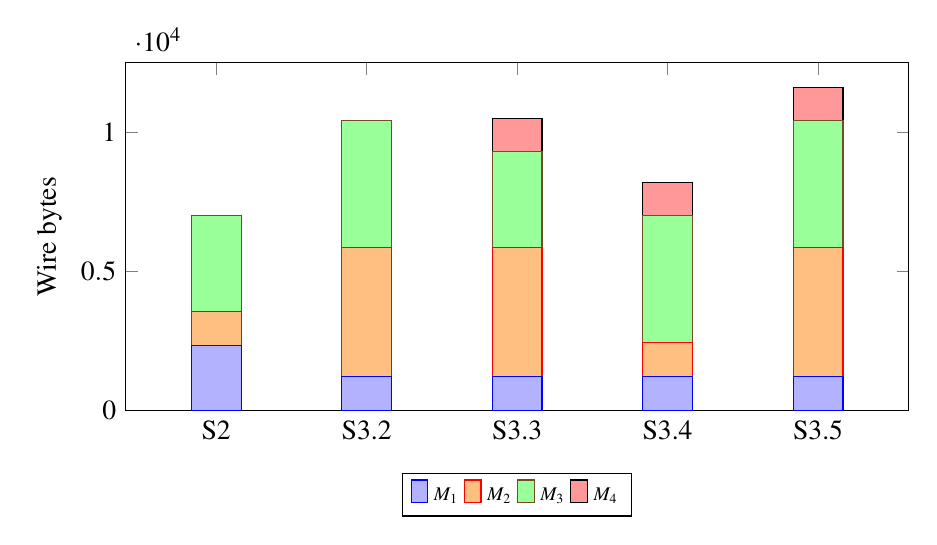
\begin{tikzpicture}
\begin{axis}[
    width=0.95\linewidth, height=6cm,
    ybar stacked, bar width=18pt,
    ymin=0, ymax=12500,
    ylabel={Wire bytes},
    symbolic x coords={S2,S3.2,S3.3,S3.4,S3.5},
    xtick=data,
    legend style={at={(0.5,-0.18)},anchor=north,legend columns=4,font=\scriptsize},
    nodes near coords align={vertical},
    every node near coord/.append style={font=\tiny},
    enlarge x limits=0.15,
]
\addplot+[fill=blue!30] coordinates {(S2,2344)(S3.2,1221)(S3.3,1221)(S3.4,1221)(S3.5,1221)};
\addplot+[fill=orange!50] coordinates {(S2,1226)(S3.2,4633)(S3.3,4633)(S3.4,1226)(S3.5,4633)};
\addplot+[fill=green!40] coordinates {(S2,3461)(S3.2,4577)(S3.3,3461)(S3.4,4577)(S3.5,4577)};
\addplot+[fill=red!40] coordinates {(S2,0)(S3.2,0)(S3.3,1176)(S3.4,1176)(S3.5,1176)};
\legend{$M_1$,$M_2$,$M_3$,$M_4$}
\end{axis}
\end{tikzpicture}
\caption{Kontribusi per-pesan terhadap total \emph{byte} kawat
(\emph{stacked}) untuk kelima varian EAP-EDHOC-PQ pada ukuran fragmen
EAP 256-\emph{byte}. \VarSecShort{2} membayar untuk
$\mathit{kem.ct}_R$ di dalam $M_1$, sementara \emph{hybrid} empat-\emph{flight}
(\VarSecShort{3.3}, \VarSecShort{3.4}, \VarSecShort{3.5}) menambahkan
$M_4$ eksplisit.}
\label{fig:wire-stacked}
\end{figure}
\FloatBarrier
Tabel~\ref{tab:processing} melaporkan rata-rata waktu \emph{handshake}
ujung-ke-ujung (dalam mikrodetik), dipecah berdasarkan \emph{deployment}
dan pihak. Total waktu \emph{handshake} (\emph{Initiator}+\emph{Responder}
digabungkan) pada jalur AAA berkisar dari sekitar $56$~ms untuk
\VarSec{3.2} hingga $440$~ms untuk \VarSec{3.4}. Dua observasi
menonjol. \emph{Pertama}, jalur AAA tidak pernah menjadi konfigurasi
tercepat-paling-lambat meski menambah satu \emph{hop} RADIUS: untuk
\VarSec{3.4} dan \VarSec{3.5}, jalur Non-EAP dan Standalone justru
lebih lambat karena kekurangan primitif perakitan-ulang fragmen yang
dioptimalkan pada \emph{server} AAA. \emph{Kedua}, \VarSec{3.2}
jauh lebih cepat dari \VarSec{2} dalam jumlah \emph{Initiator}/\emph{Responder}
($56$~ms berbanding $131$~ms pada AAA), karena \VarSec{2} menggunakan
Pesan\,3 yang sangat besar ($3{,}461$ \emph{byte}) yang memerlukan
$14$ fragmen, sedangkan \VarSec{3.2} memakai ulang Pesan\,1 yang
ringkas.

\begin{table}[h]
\centering
\footnotesize
\caption{Rata-rata waktu pemrosesan ujung-ke-ujung per \emph{handshake}
dalam mikrodetik ($\mu$s), berdasarkan \emph{deployment} dan peran.
``Sum'' adalah \emph{Initiator}+\emph{Responder}.}
\label{tab:processing}
\begin{tabular}{lrrrrrrrrr}
\toprule
& \multicolumn{3}{c}{\textbf{AAA (FreeRADIUS)}} & \multicolumn{3}{c}{\textbf{EAP-Standalone}} & \multicolumn{3}{c}{\textbf{Non-EAP}} \\
\cmidrule(lr){2-4}\cmidrule(lr){5-7}\cmidrule(lr){8-10}
\textbf{Varian} & Init & Resp & Sum & Init & Resp & Sum & Init & Resp & Sum \\
\midrule
\VarSecShort{2}   &  64{,}505 &  66{,}870 & 131{,}375 &  65{,}621 &  68{,}578 & 134{,}199 &  69{,}038 &  71{,}971 & 141{,}009 \\
\VarSecShort{3.2} &  28{,}051 &  28{,}130 &  56{,}181 &  35{,}668 &  35{,}715 &  71{,}383 &  32{,}133 &  33{,}524 &  65{,}657 \\
\VarSecShort{3.3} & 172{,}086 & 186{,}444 & 358{,}530 & 173{,}831 & 187{,}152 & 360{,}982 & 165{,}068 & 151{,}258 & 316{,}326 \\
\VarSecShort{3.4} & 219{,}917 & 220{,}463 & 440{,}379 & 236{,}108 & 245{,}434 & 481{,}543 & 241{,}271 & 241{,}371 & 482{,}641 \\
\VarSecShort{3.5} & 184{,}496 & 180{,}137 & 364{,}633 & 213{,}043 & 211{,}815 & 424{,}859 & 192{,}235 & 194{,}671 & 386{,}906 \\
\bottomrule
\end{tabular}
\end{table}

% --- Line chart: total handshake time across deployments ---
\begin{figure}[H]
\centering
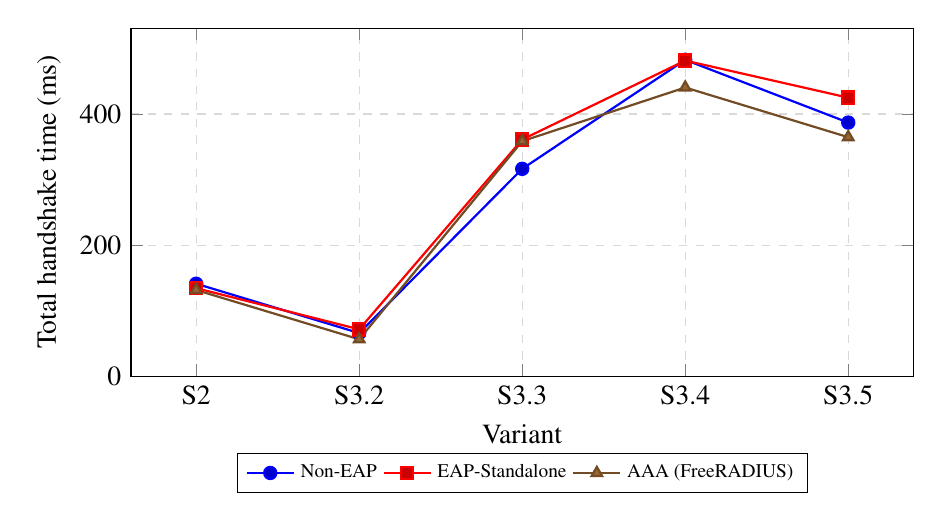
\begin{tikzpicture}
\begin{axis}[
    width=0.95\linewidth, height=6cm,
    ylabel={Total handshake time (ms)},
    xlabel={Variant},
    symbolic x coords={S2,S3.2,S3.3,S3.4,S3.5},
    xtick=data,
    ymin=0,
    legend style={at={(0.5,-0.22)},anchor=north,legend columns=3,font=\scriptsize},
    grid=both, grid style={dashed,gray!30},
    mark options={scale=1.1},
]
\addplot+[mark=*,thick] coordinates {(S2,141.0)(S3.2,65.7)(S3.3,316.3)(S3.4,482.6)(S3.5,386.9)};
\addplot+[mark=square*,thick] coordinates {(S2,134.2)(S3.2,71.4)(S3.3,361.0)(S3.4,481.5)(S3.5,424.9)};
\addplot+[mark=triangle*,thick] coordinates {(S2,131.4)(S3.2,56.2)(S3.3,358.5)(S3.4,440.4)(S3.5,364.6)};
\legend{Non-EAP, EAP-Standalone, AAA (FreeRADIUS)}
\end{axis}
\end{tikzpicture}
\caption{Waktu \emph{handshake} ujung-ke-ujung per varian pada ketiga
\emph{deployment}. Kurva saling berpotongan antara varian tiga-\emph{flight}
dan empat-\emph{flight}; jalur AAA berbasis-FreeRADIUS kompetitif
dengan EAP-Standalone untuk setiap varian.}
\label{fig:handshake-line}
\end{figure}
\FloatBarrier
Tabel~\ref{tab:overhead} melaporkan dekomposisi waktu \emph{handshake}
\emph{wall-clock} menjadi waktu CPU (komputasi), waktu tunggu I/O
($\mathit{io\_wait}$), dan \emph{overhead} residual (pembingkaian,
memcpy, mesin keadaan fragmentasi). Rasio CPU-terhadap-\emph{wall-clock}
konsisten di bawah $25\%$ pada semua varian, yang berarti sebagian
besar waktu \emph{wall-clock} \emph{handshake} dihabiskan menunggu
jaringan dan perakitan-ulang fragmen --- konsekuensi langsung dari
fragmentasi \emph{lock-step} EAP pada granularitas 256-\emph{byte}.
Memori puncak RSS sekitar $2.1$--$2.2$~MB untuk ketiga \emph{deployment},
menegaskan bahwa skema dapat di-\emph{deploy} pada perangkat IoT
kelas~2 tipikal.

\begin{table}[h]
\centering
\footnotesize
\caption{Waktu CPU, tunggu I/O, \emph{overhead} residual, dan rasio
CPU/\emph{wall} untuk \emph{deployment} AAA. Semua waktu dalam
mikrodetik.}
\label{tab:overhead}
\begin{tabular}{llrrrrr}
\toprule
\textbf{Varian} & \textbf{Peran} & \textbf{CPU ($\mu$s)} & \textbf{\emph{Wall} ($\mu$s)} & \textbf{Tunggu I/O} & \textbf{Residual} & \textbf{CPU/\emph{Wall}} \\
\midrule
\VarSecShort{2}   & Init &  5{,}623 &  64{,}505 &  50{,}103 &   8{,}834 & 0.087 \\
\VarSecShort{2}   & Resp &  1{,}750 &  66{,}870 &   3{,}074 &  62{,}155 & 0.026 \\
\VarSecShort{3.2} & Init &  7{,}029 &  28{,}051 &   7{,}688 &  13{,}405 & 0.251 \\
\VarSecShort{3.2} & Resp &  5{,}929 &  28{,}130 &   1{,}920 &  20{,}482 & 0.211 \\
\VarSecShort{3.3} & Init &  5{,}025 & 172{,}086 &  58{,}156 & 108{,}989 & 0.029 \\
\VarSecShort{3.3} & Resp & 13{,}336 & 186{,}444 & 101{,}110 &  72{,}365 & 0.072 \\
\VarSecShort{3.4} & Init &  5{,}170 & 219{,}917 & 101{,}312 & 113{,}511 & 0.024 \\
\VarSecShort{3.4} & Resp &  6{,}812 & 220{,}463 &  96{,}770 & 117{,}272 & 0.031 \\
\VarSecShort{3.5} & Init & 10{,}252 & 184{,}496 &  58{,}130 & 116{,}219 & 0.056 \\
\VarSecShort{3.5} & Resp & 14{,}866 & 180{,}137 &  86{,}543 &  79{,}184 & 0.083 \\
\bottomrule
\end{tabular}
\end{table}

% --- Horizontal stacked bar: CPU vs IO-wait vs residual per (variant,role) ---
\begin{figure}[H]
\centering
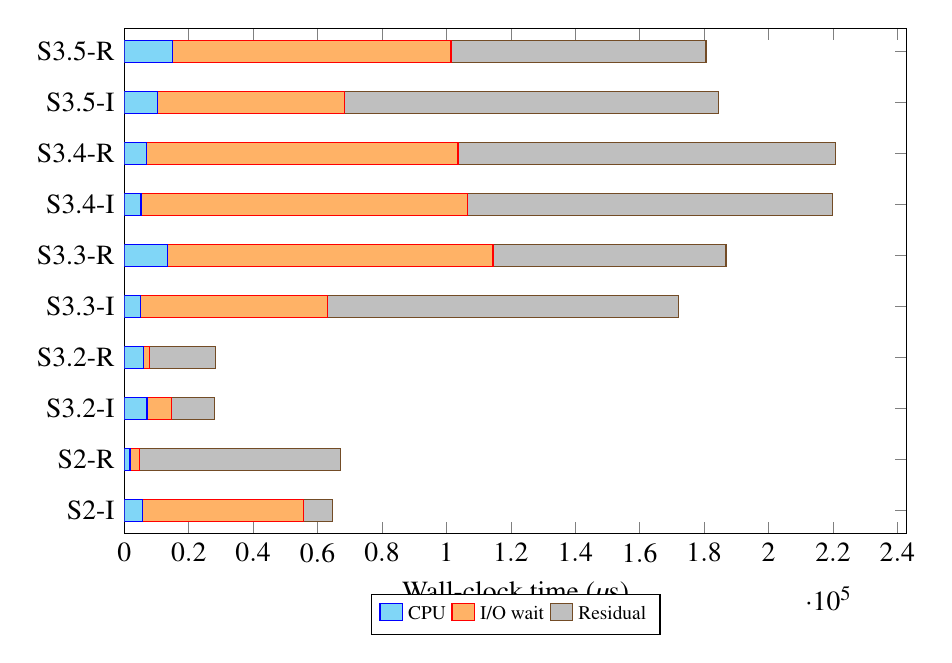
\begin{tikzpicture}
\begin{axis}[
    width=0.95\linewidth, height=8cm,
    xbar stacked, bar width=8pt,
    xmin=0,
    xlabel={Wall-clock time ($\mu$s)},
    symbolic y coords={S2-I,S2-R,S3.2-I,S3.2-R,S3.3-I,S3.3-R,S3.4-I,S3.4-R,S3.5-I,S3.5-R},
    ytick=data,
    legend style={at={(0.5,-0.12)},anchor=north,legend columns=3,font=\scriptsize},
    enlarge y limits=0.05,
    every axis plot/.append style={draw=black!40},
]
\addplot+[fill=cyan!50] coordinates {
  (5623,S2-I)(1750,S2-R)(7029,S3.2-I)(5929,S3.2-R)
  (5025,S3.3-I)(13336,S3.3-R)(5170,S3.4-I)(6812,S3.4-R)
  (10252,S3.5-I)(14866,S3.5-R)};
\addplot+[fill=orange!60] coordinates {
  (50103,S2-I)(3074,S2-R)(7688,S3.2-I)(1920,S3.2-R)
  (58156,S3.3-I)(101110,S3.3-R)(101312,S3.4-I)(96770,S3.4-R)
  (58130,S3.5-I)(86543,S3.5-R)};
\addplot+[fill=gray!50] coordinates {
  (8834,S2-I)(62155,S2-R)(13405,S3.2-I)(20482,S3.2-R)
  (108989,S3.3-I)(72365,S3.3-R)(113511,S3.4-I)(117272,S3.4-R)
  (116219,S3.5-I)(79184,S3.5-R)};
\legend{CPU, I/O wait, Residual}
\end{axis}
\end{tikzpicture}
\caption{Dekomposisi \emph{wall-clock} menjadi CPU, tunggu I/O, dan
\emph{overhead} residual untuk setiap (varian, peran) pada
\emph{deployment} AAA. Pita CPU seragam tipis: kriptografi tertutup
oleh latensi fragmentasi pada setiap konfigurasi.}
\label{fig:overhead-stacked}
\end{figure}
\FloatBarrier
Tabel~\ref{tab:operations} melaporkan total waktu per \emph{handshake}
yang dihabiskan pada setiap operasi primitif, diukur pada
\emph{deployment} AAA. Pembangkitan tanda tangan sejauh ini
menjadi kontributor kriptografi terbesar (umumnya $2{,}165$--$8{,}822$
$\mu$s per pemanggilan) dan mendominasi anggaran kriptografi untuk
setiap varian yang menggunakan ML-DSA. ML-KEM $\KemKeyGen$, $\Encaps$,
dan $\Decaps$ relatif murah, masing-masing dalam rentang
$230$--$2{,}035$~$\mu$s. Pada setiap varian, kriptografi menyumbang
jauh lebih sedikit daripada tunggu I/O akibat fragmen, memperkuat
kesimpulan dari Tabel~\ref{tab:overhead} bahwa \emph{fragmentasi,
bukan kriptografi, mendominasi biaya \emph{wall-clock} EAP-EDHOC-PQ
pada rezim fragmen 256-\emph{byte}.}

\begin{table}[h]
\centering
\footnotesize
\caption{Total waktu kriptografi per \emph{handshake} (dalam $\mu$s)
pada \emph{deployment} AAA. Tanda strip (---) menunjukkan operasi
tidak dipanggil oleh varian pada peran tersebut.}
\label{tab:operations}
\begin{tabular}{llrrrrrrr}
\toprule
\textbf{Varian} & \textbf{Peran} & \textbf{KeyGen} & \textbf{Encaps} & \textbf{Decaps} & \textbf{Sign} & \textbf{Verify} & \textbf{HKDF} & \textbf{AEAD} \\
\midrule
\VarSecShort{2}   & Init & 370 &    472 &  608 & 4{,}067 & ---       &  20 &  13 \\
\VarSecShort{2}   & Resp & 232 &    283 &  345 & ---     &    697    &  17 &  46 \\
\VarSecShort{3.2} & Init & 374 &    470 &  609 & 4{,}337 &    943    & 205 &   9 \\
\VarSecShort{3.2} & Resp & 376 &    413 &  631 & 2{,}830 & 1{,}181   & 225 &  56 \\
\VarSecShort{3.3} & Init & 370 & ---    & 1{,}215 & 2{,}165 &    942 & 210 &  10 \\
\VarSecShort{3.3} & Resp & 805 & 1{,}520 & ---    & 8{,}822 & 1{,}380 & 310 &  72 \\
\VarSecShort{3.4} & Init & 371 &    470 & 1{,}218 & 2{,}968 & ---     &  25 &  11 \\
\VarSecShort{3.4} & Resp & 731 & 1{,}776 & 1{,}234 & ---     & 2{,}424 &  75 & 112 \\
\VarSecShort{3.5} & Init & 371 &    473 & 1{,}223 & 6{,}885 &    943  & 211 &  11 \\
\VarSecShort{3.5} & Resp & 906 & 2{,}034 & 1{,}224 & 7{,}163 & 2{,}445 & 445 & 118 \\
\bottomrule
\end{tabular}
\end{table}

% --- Polar / radar plot: per-operation cost shape per variant (Responder) ---
\begin{figure}[H]
\centering
\begin{tikzpicture}
\begin{polaraxis}[
    width=0.85\linewidth, height=8cm,
    xtick={0,51.43,...,308.57},
    xticklabels={KeyGen,Encaps,Decaps,Sign,Verify,HKDF,AEAD},
    ymin=0, ymax=10000,
    ytick={2000,4000,6000,8000},
    yticklabel style={font=\tiny},
    xticklabel style={font=\tiny},
    legend style={at={(1.25,1.0)},anchor=north west,font=\scriptsize},
]
% S2 (Resp): 232,283,345,0,697,17,46
\addplot+[mark=*] coordinates {(0,232)(51.43,283)(102.86,345)(154.29,0)(205.71,697)(257.14,17)(308.57,46)(360,232)};
% S3.2: 376,413,631,2830,1181,225,56
\addplot+[mark=square*] coordinates {(0,376)(51.43,413)(102.86,631)(154.29,2830)(205.71,1181)(257.14,225)(308.57,56)(360,376)};
% S3.3: 805,1520,0,8822,1380,310,72
\addplot+[mark=triangle*] coordinates {(0,805)(51.43,1520)(102.86,0)(154.29,8822)(205.71,1380)(257.14,310)(308.57,72)(360,805)};
% S3.4: 731,1776,1234,0,2424,75,112
\addplot+[mark=diamond*] coordinates {(0,731)(51.43,1776)(102.86,1234)(154.29,0)(205.71,2424)(257.14,75)(308.57,112)(360,731)};
% S3.5: 906,2034,1224,7163,2445,445,118
\addplot+[mark=pentagon*] coordinates {(0,906)(51.43,2034)(102.86,1224)(154.29,7163)(205.71,2445)(257.14,445)(308.57,118)(360,906)};
\legend{S2,S3.2,S3.3,S3.4,S3.5}
\end{polaraxis}
\end{tikzpicture}
\caption{Biaya kriptografi per-operasi (sisi \emph{Responder},
\emph{deployment} AAA), digambar sebagai \emph{radar plot}. Varian
yang mengandalkan ML-DSA (\VarSecShort{3.3} dan \VarSecShort{3.5})
memanjang sepanjang \emph{spoke} \textsc{Sign}; \VarSecShort{3.4}
justru memanjang sepanjang \textsc{Encaps}/\textsc{Decaps}/\textsc{Verify}.}
\label{fig:ops-radar}
\end{figure}
\FloatBarrier

%-------------------------------------------------------------------------
\subsection{Konsumsi Energi}
\label{sec:energy}
%-------------------------------------------------------------------------
Pengukuran \emph{wall-clock} saja tidak menangkap dampak fragmentasi
EAP pada \emph{endpoint} IoT \emph{bertenaga-baterai}, yang
mendominasi \emph{deployment} \emph{e-business} seperti mesin penjual
otomatis nirkabel dan \emph{node} sensor bertenaga-baterai. Kami
karena itu menggunakan waktu per-\emph{handshake} dari
Tabel~\ref{tab:overhead} untuk menurunkan estimasi energi orde-pertama
yang transparan. Kami mengadopsi model yang sengaja sederhana agar
asumsinya dapat diaudit; kami tidak mengklaim akurasi sub-mJ.

\paragraph{Model.} Untuk satu \emph{handshake} kami mengaproksimasi
energi per-peran sebagai jumlah tiga komponen aditif,
\begin{equation}
E_{\mathrm{hs}} \;=\; P_{\mathrm{cpu}}\cdot t_{\mathrm{cpu}}
\;+\; P_{\mathrm{idle}}\cdot t_{\mathrm{io}}
\;+\; P_{\mathrm{tx}}\cdot \frac{8\,B_{\mathrm{wire}}}{R_{\mathrm{tx}}},
\label{eq:energy}
\end{equation}
di mana $t_{\mathrm{cpu}}$ adalah waktu CPU dari
Tabel~\ref{tab:overhead}, $t_{\mathrm{io}}$ adalah waktu tunggu I/O
dari tabel yang sama, $B_{\mathrm{wire}}$ adalah \emph{byte} kawat
per-peran dari Tabel~\ref{tab:frag}, dan $R_{\mathrm{tx}}$ adalah
\emph{bit-rate} \emph{link}. Nilai daya referensi tipikal untuk
\emph{node} IoT kelas ARM Cortex-M dengan radio berdaya-rendah:
$P_{\mathrm{cpu}}\!=\!48$~mW (aktif),
$P_{\mathrm{idle}}\!=\!4$~mW (MCU \emph{light-sleep} menunggu radio),
$P_{\mathrm{tx}}\!=\!60$~mW (radio dalam TX/RX), dan
$R_{\mathrm{tx}}\!=\!250$~kbps (\emph{throughput} kelas IEEE~802.15.4).
Nilai-nilai ini berada dalam rentang yang dilaporkan karakterisasi
IoT yang banyak dikutip~\cite{FVW24,FTK+25} dan dinyatakan eksplisit
sehingga tabel dapat diskalakan ulang oleh pembaca untuk platform
yang berbeda: di bawah~\eqref{eq:energy}, $E_{\mathrm{hs}}$ berskala
linier dalam setiap $P_*$ dan berbanding terbalik dalam
$R_{\mathrm{tx}}$.

\paragraph{Hasil.} Tabel~\ref{tab:energy} melaporkan estimasi energi
per-peran menggunakan \eqref{eq:energy} pada \emph{deployment} AAA.
Total energi per-\emph{handshake} berkisar dari $\approx\!4$~mJ untuk
\VarSecShort{3.2} hingga $\approx\!22$~mJ untuk \VarSecShort{3.4}, dan
porsi yang dapat diatribusikan ke CPU paling banyak $\approx\!13\%$.
Porsi dominan adalah suku tunggu I/O, mengonfirmasi pada level energi
kesimpulan terikat-fragmentasi yang sudah ditarik dari
Tabel~\ref{tab:overhead}.

\begin{table}[H]
\centering
\footnotesize
\caption{Estimasi energi per-\emph{handshake} orde-pertama dari
\eqref{eq:energy} pada \emph{deployment} AAA, dalam milijoule.
Parameter referensi: $P_{\mathrm{cpu}}\!=\!48$~mW, $P_{\mathrm{idle}}\!=\!4$~mW,
$P_{\mathrm{tx}}\!=\!60$~mW, $R_{\mathrm{tx}}\!=\!250$~kbps.
$E_{\mathrm{cpu}}\!=\!P_{\mathrm{cpu}} t_{\mathrm{cpu}}$,
$E_{\mathrm{io}}\!=\!P_{\mathrm{idle}} t_{\mathrm{io}}$,
$E_{\mathrm{tx}}\!=\!P_{\mathrm{tx}}\!\cdot\!8B_{\mathrm{wire}}/R_{\mathrm{tx}}$.
\emph{Byte} kawat dipecah per-peran menggunakan Tabel~\ref{tab:frag}
($M_1,M_3$ dari $I$, $M_2,M_4$ dari $R$).}
\label{tab:energy}
\begin{tabular}{llrrrr}
\toprule
\textbf{Varian} & \textbf{Peran} & $E_{\mathrm{cpu}}$ (mJ) & $E_{\mathrm{io}}$ (mJ) & $E_{\mathrm{tx}}$ (mJ) & $E_{\mathrm{hs}}$ (mJ) \\
\midrule
\VarSecShort{2}   & Init & 0.27 & 0.20 & 1.11 &  1.58 \\
\VarSecShort{2}   & Resp & 0.08 & 0.01 & 0.24 &  0.33 \\
\VarSecShort{3.2} & Init & 0.34 & 0.03 & 1.11 &  1.48 \\
\VarSecShort{3.2} & Resp & 0.28 & 0.01 & 0.89 &  1.18 \\
\VarSecShort{3.3} & Init & 0.24 & 0.23 & 0.90 &  1.37 \\
\VarSecShort{3.3} & Resp & 0.64 & 0.40 & 1.12 &  2.16 \\
\VarSecShort{3.4} & Init & 0.25 & 0.41 & 1.11 &  1.77 \\
\VarSecShort{3.4} & Resp & 0.33 & 0.39 & 0.46 &  1.18 \\
\VarSecShort{3.5} & Init & 0.49 & 0.23 & 1.11 &  1.83 \\
\VarSecShort{3.5} & Resp & 0.71 & 0.35 & 1.12 &  2.18 \\
\midrule
\VarSecShort{2}   & Sum  & 0.35 & 0.21 & 1.35 &  1.91 \\
\VarSecShort{3.2} & Sum  & 0.62 & 0.04 & 2.00 &  2.66 \\
\VarSecShort{3.3} & Sum  & 0.88 & 0.63 & 2.02 &  3.53 \\
\VarSecShort{3.4} & Sum  & 0.58 & 0.80 & 1.57 &  2.95 \\
\VarSecShort{3.5} & Sum  & 1.20 & 0.58 & 2.23 &  4.01 \\
\bottomrule
\end{tabular}
\end{table}

% --- Grouped bar: per-role energy split (CPU vs IO vs TX) ---
\begin{figure}[H]
\centering
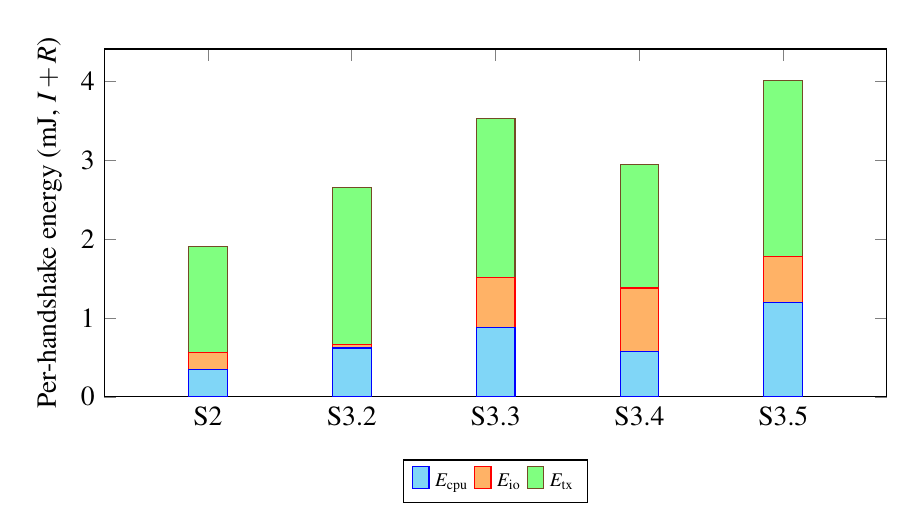
\begin{tikzpicture}
\begin{axis}[
    width=0.95\linewidth, height=6cm,
    ybar stacked, bar width=14pt,
    ymin=0,
    ylabel={Per-handshake energy (mJ, $I+R$)},
    symbolic x coords={S2,S3.2,S3.3,S3.4,S3.5},
    xtick=data,
    legend style={at={(0.5,-0.18)},anchor=north,legend columns=3,font=\scriptsize},
    enlarge x limits=0.18,
]
\addplot+[fill=cyan!50] coordinates {(S2,0.35)(S3.2,0.62)(S3.3,0.88)(S3.4,0.58)(S3.5,1.20)};
\addplot+[fill=orange!60] coordinates {(S2,0.21)(S3.2,0.04)(S3.3,0.63)(S3.4,0.80)(S3.5,0.58)};
\addplot+[fill=green!50] coordinates {(S2,1.35)(S3.2,2.00)(S3.3,2.02)(S3.4,1.57)(S3.5,2.23)};
\legend{$E_{\mathrm{cpu}}$,$E_{\mathrm{io}}$,$E_{\mathrm{tx}}$}
\end{axis}
\end{tikzpicture}
\caption{Estimasi energi per-\emph{handshake} ($I\!+\!R$) di bawah
\eqref{eq:energy}. Suku transmisi $E_{\mathrm{tx}}$ mengikuti
\emph{byte} kawat \emph{stacked} dari Fig.~\ref{fig:wire-stacked},
sementara kontribusi CPU tetap menjadi porsi minor untuk setiap
varian.}
\label{fig:energy-stacked}
\end{figure}
\FloatBarrier


%=========================================================================
\section{Pembahasan}
\label{discussion}
%=========================================================================
Hasil kami mengarah pada beberapa observasi dengan konsekuensi
praktis.

\paragraph{Fragmentasi, bukan kriptografi, mendorong waktu \emph{wall-clock}.}
Pada setiap varian dan setiap \emph{deployment}, rasio
CPU-terhadap-\emph{wall-clock} tetap di bawah~$0.25$. Waktu tunggu
I/O untuk fragment-ACK saja menyumbang $50$--$60\%$ dari total waktu
\emph{handshake} untuk varian empat-\emph{flight}. Menaikkan ukuran
fragmen EAP di atas $1024$ \emph{byte} --- yang sudah diizinkan
RFC~3748 ketika lapisan bawah mendukungnya --- secara mekanis akan
memotong jumlah fragmen empat kali lipat, dan kami menduga akan
mengurangi waktu \emph{wall-clock} \emph{handshake} secara
proporsional.

\paragraph{Otentikasi \emph{Responder} yang ditangguhkan (\texorpdfstring{\VarSec{3.4}}{Section 3.4}) menarik.}
Meskipun merupakan \emph{hybrid} empat-\emph{flight} dengan Pesan\,3
terbesar ($4{,}577$ \emph{byte}), \VarSec{3.4} menjaga total \emph{byte}
kawat pada $8{,}207$ dan total fragmen pada~$34$, jauh lebih kecil
daripada \VarSec{3.2}, \VarSec{3.3}, dan \VarSec{3.5}. Harganya adalah
\emph{Initiator} tidak dapat menerima otentikasi \emph{Responder}
sampai Pesan\,4. Untuk akses jaringan EAP ini adalah \emph{trade-off}
yang baik: EAP-Success bagaimanapun hanya dikirim setelah Pesan\,4.

\paragraph{\texorpdfstring{\VarSec{2}}{Section 2} adalah \emph{default} yang tepat untuk lingkungan yang memercayai KEM.}
Jika \emph{deployment} sudah mendistribusikan kunci publik KEM
\emph{Responder} (mis., melalui kredensial \emph{onboarding}
ter-pra-provisi), \VarSec{2} menghasilkan jejak kawat terkecil dan
menggunakan satu tanda tangan ML-DSA (alih-alih dua), untuk
\emph{handshake} tiga-\emph{flight} bersih yang memetakan secara
natif ke pola \emph{request}/\emph{response} EAP.

\paragraph{AAA tidak selalu memperlambat.}
Bertentangan dengan intuisi, \emph{deployment} AAA berbasis-FreeRADIUS
bukan yang paling lambat dalam pengukuran kami; untuk \VarSec{3.4}
sebenarnya $\sim\!10\%$ lebih cepat dari EAP-Standalone. Kami
mengatribusikan ini pada paketisasi RADIUS yang efisien dari
FreeRADIUS dan jalur I/O \emph{batched}-nya, yang mengompensasi
\emph{hop} RADIUS tambahan. Ini hasil yang menggembirakan untuk
\emph{deployment} produksi.

\paragraph{Energi mengikuti kawat, bukan CPU.}
Model energi orde-pertama dari Section~\ref{sec:energy} memeringkat
kelima varian pada urutan yang esensinya sama dengan total \emph{byte}
kawat dan jumlah fragmennya: $E_{\mathrm{tx}}$ dan $E_{\mathrm{io}}$
bersama-sama mendominasi $E_{\mathrm{cpu}}$ untuk setiap varian
(Tabel~\ref{tab:energy}). Untuk \emph{endpoint} \emph{e-business}
bertenaga-baterai seperti terminal penjual nirkabel atau pelacak aset,
ini berarti memilih varian yang lebih kecil di kawat (\VarSecShort{2}
atau \VarSecShort{3.4}) menghasilkan keuntungan baterai lebih besar
daripada memilih primitif yang lebih ringan secara kriptografis pada
level parameter yang sama.

\paragraph{Keterbatasan dan kerja mendatang.}
Pengukuran kami menggunakan ML-KEM-768/ML-DSA-44 dan ukuran fragmen
256-\emph{byte}; mengevaluasi himpunan parameter Level\,3 dan
Level\,5, ukuran fragmen lebih besar, dan lapisan bawah nirkabel
\emph{lossy} (mis., 802.15.4, LoRaWAN) ditinggalkan untuk kerja
mendatang. Model ProVerif kami memperlakukan ML-KEM sebagai KEM
IND-CCA2 yang diidealkan; analisis komputasional sejalan
dengan~\cite{Fer24,GM23} masih terbuka.


%=========================================================================
\section{Kesimpulan}
\label{conclusion}
%=========================================================================
Kami telah menyajikan EAP-EDHOC-PQ, spesifikasi terpadu yang membawa
lima mode otentikasi pasca-kuantum EDHOC --- \VarSec{2}, \VarSec{3.2},
\VarSec{3.3}, \VarSec{3.4} dan \VarSec{3.5} --- ke dalam kerangka
EAP, dan kami mengevaluasinya secara formal dalam ProVerif maupun
empiris pada \emph{deployment} Non-EAP, EAP-Standalone, dan AAA
berbasis-FreeRADIUS. Kelima varian memenuhi otentikasi mutual,
kerahasiaan kunci sesi, \emph{forward secrecy}, dan ketahanan
\emph{replay}. Secara empiris, \VarSec{3.2} adalah varian
tiga-\emph{flight} tercepat, \VarSec{2} adalah yang terkecil di kawat,
dan \VarSec{3.4} menawarkan \emph{trade-off} terbaik di antara mode
\emph{hybrid} empat-\emph{flight} berkat otentikasi \emph{Responder}
yang ditangguhkan. Model energi orde-pertama yang diturunkan dari
pengukuran yang sama menunjukkan bahwa anggaran energi
per-\emph{handshake} pada \emph{node} kelas-IoT tipikal didominasi
oleh transmisi dan tunggu I/O alih-alih kriptografi, sehingga
mengoptimalkan ukuran fragmen EAP yang dinegosiasikan adalah tuas
yang lebih berdampak untuk metode PQ-EAP mendatang dibandingkan
mempercepat KEM yang mendasarinya. Temuan ini, meski terbatas pada
himpunan parameter dan kecepatan \emph{link} yang kami ukur, menggambar
titik awal praktis untuk otentikasi akses jaringan tahan-kuantum bagi
\emph{endpoint} IoT terhubung-Wi-Fi pada \emph{deployment} \emph{e-business}
seperti mesin penjual otomatis berjaringan, \emph{beacon}
\emph{smart-retail}, dan sensor logistik terhubung.


\label{sect:bib}
\bibliographystyle{unsrt}
\bibliography{reference}

\end{document}